% !TeX program = xelatex
% !TeX encoding = UTF-8
% Spedizione P02 · Foraminiferi, coppe e campagne
% Presentazione della spedizione P02 nella serie planetaria di GeoStat Lab.
% Compilazione: xelatex -interaction=nonstopmode P02_Foraminiferi.tex (due passaggi)
% 32 slide. Diagrammi TikZ, figure vettoriali da R/P02_figure.R, codice R, dati ed esperimenti inclusi.
\RequirePackage{fix-cm}
\documentclass[12pt,aspectratio=1610]{beamer}
\geometry{paperwidth=20cm,paperheight=12.5cm}
\usepackage[italian,provide=*]{babel}
\usepackage{fontspec,adjustbox,tabularx}
\IfFontExistsTF{NimbusSans-Regular.otf}{
\setsansfont{NimbusSans-Regular.otf}[BoldFont=NimbusSans-Bold.otf,ItalicFont=NimbusSans-Italic.otf,BoldItalicFont=NimbusSans-BoldItalic.otf]
\setmainfont{NimbusSans-Regular.otf}[BoldFont=NimbusSans-Bold.otf,ItalicFont=NimbusSans-Italic.otf,BoldItalicFont=NimbusSans-BoldItalic.otf]
}{
\setsansfont{TeX Gyre Heros}
\setmainfont{TeX Gyre Heros}
}
\IfFontExistsTF{DejaVu Sans Mono}{
\setmonofont{DejaVu Sans Mono}[Scale=.88]
}{\setmonofont{Latin Modern Mono}[Scale=.88]}
\usefonttheme{professionalfonts}
\usepackage{amsmath,amssymb,booktabs,array,graphicx,tikz,bookmark}
\usetikzlibrary{calc,positioning,arrows.meta}
\graphicspath{{Figure/}}
\definecolor{Paper}{HTML}{F8F6F1}
\definecolor{Ink}{HTML}{253344}
\definecolor{Navy}{HTML}{15283E}
\definecolor{Quantum}{HTML}{5146A5}
\definecolor{Classical}{HTML}{087C74}
\definecolor{Muted}{HTML}{657180}
\definecolor{Rule}{HTML}{D6DAD9}
\definecolor{Night}{HTML}{112236}
\definecolor{Lilac}{HTML}{ABB5FF}
\definecolor{Mint}{HTML}{72D8C8}
\setbeamercolor{background canvas}{bg=Paper}
\setbeamercolor{normal text}{fg=Ink}
\setbeamertemplate{navigation symbols}{}
\setbeamertemplate{headline}{}
\setbeamertemplate{footline}{}
\setbeamersize{text margin left=0pt,text margin right=0pt}
\hypersetup{colorlinks=true,linkcolor=Classical,urlcolor=Classical,pdfpagemode=UseOutlines,pdfstartview=Fit,
 pdftitle={Spedizione P02 · Foraminiferi, coppe e campagne},pdfauthor={GeoStat Lab · materiali di Marzio De Corato},
 pdfsubject={GeoStat Lab · P02}}
\bookmarksetup{open,openlevel=0,depth=2}
\newsavebox{\BodyBox}
\newsavebox{\SideBox}
\newsavebox{\RecallBox}
\newsavebox{\TitleBox}
\newcommand{\MeasureBox}[2]{\typeout{REVIEWBOX:#1:\the\wd#2:\the\ht#2:\the\dp#2}}

% Revisione completa: diagrammi TikZ, formalismo e box R.
\usepackage[most]{tcolorbox}
\usepackage{listings}
\usetikzlibrary{fit,backgrounds,matrix,decorations.pathreplacing}
\definecolor{GeoA}{HTML}{1D7890}
\definecolor{GeoB}{HTML}{C57E42}
\definecolor{GeoC}{HTML}{7363AA}
\definecolor{GeoTint}{HTML}{F0F4F3}
\lstdefinestyle{GeoR}{language=R,basicstyle=\ttfamily\fontsize{9.2}{12.2}\selectfont,
 keywordstyle=\color{Quantum}\bfseries,commentstyle=\color{Classical},stringstyle=\color{GeoB},
 numbers=left,numberstyle=\tiny\color{Muted},numbersep=4pt,showstringspaces=false,
 columns=fullflexible,keepspaces=true,breaklines=true,xleftmargin=1.15em,
 frame=none,aboveskip=0pt,belowskip=0pt,tabsize=2}
\newsavebox{\PilotLeftBox}
\newsavebox{\PilotRightBox}
\newcommand{\PLabel}[1]{\par{\color{Classical}\bfseries\fontsize{9}{11}\selectfont\MakeUppercase{#1}}\par\vspace{1.8mm}}
\newcommand{\PBody}[1]{\par{\fontsize{11.3}{14.8}\selectfont #1\par}}
\newcommand{\PSmall}[1]{\par{\fontsize{9.8}{13.1}\selectfont #1\par}}
\newcommand{\PCode}[2]{%
\begin{tcolorbox}[enhanced,arc=1.8mm,boxrule=.65pt,
  colback=white,colframe=Classical!75!Navy,colbacktitle=Navy,
  coltitle=white,fonttitle=\bfseries\fontsize{9.6}{12}\selectfont,
  title={#1},left=1.7mm,right=1.3mm,top=1.5mm,bottom=1.3mm,
  before skip=1mm,after skip=1mm]
\lstinputlisting[style=GeoR]{Codice/#2}
\end{tcolorbox}}
\newcommand{\PInfo}[1]{%
\begin{tcolorbox}[enhanced,arc=1.6mm,boxrule=.55pt,colback=GeoTint,
 colframe=Rule!80!Classical,left=2.3mm,right=2.3mm,top=2mm,bottom=2mm,
 before skip=1mm,after skip=1mm]
\PSmall{#1}\end{tcolorbox}}
\tikzset{
 pFlow/.style={draw=Classical!45,fill=white,rounded corners=2mm,
  line width=.7pt,align=center,minimum height=1.1cm,font=\sffamily\fontsize{10}{12}\selectfont},
 pEdge/.style={-{Latex[length=2.3mm]},draw=Classical,line width=.95pt},
 pGroup/.style={draw=Rule,fill=white,rounded corners=2mm,line width=.65pt},
 pDotA/.style={circle,fill=GeoA,inner sep=1.25pt},
 pDotB/.style={circle,fill=GeoB,inner sep=1.25pt},
 pDotC/.style={circle,fill=GeoC,inner sep=1.25pt}
}
\newcommand{\PilotChrome}[4]{%
  \node[anchor=north west,inner sep=0,text width=17.7cm] at ([xshift=.95cm,yshift=-.55cm]current page.north west) {\color{Navy}\bfseries\fontsize{20.6}{24.5}\selectfont #1};
  \node[anchor=north east,inner sep=0] at ([xshift=19.05cm,yshift=-.14cm]current page.north west) {\color{Classical}\fontsize{8}{10}\selectfont\hyperlink{slide2}{#2}};
  \draw[Classical,line width=1.2pt] ([xshift=.95cm,yshift=-1.7cm]current page.north west)--([xshift=2.35cm,yshift=-1.7cm]current page.north west);
  \draw[Rule,line width=.65pt] ([xshift=.95cm,yshift=-10.36cm]current page.north west)--([xshift=19.05cm,yshift=-10.36cm]current page.north west);
  \node[anchor=north west,inner sep=0] at ([xshift=.96cm,yshift=-10.55cm]current page.north west) {\color{Classical}\bfseries\fontsize{9.1}{12}\selectfont DA RICORDARE};
  \node[anchor=north west,inner sep=0,text width=14.3cm] at ([xshift=4.2cm,yshift=-10.53cm]current page.north west) {\color{Ink}\fontsize{10.3}{13.8}\selectfont #4};
  \draw[Rule,line width=.35pt] ([xshift=.95cm,yshift=-11.92cm]current page.north west)--([xshift=19.05cm,yshift=-11.92cm]current page.north west);
  \node[anchor=north west,inner sep=0] at ([xshift=.95cm,yshift=-12.06cm]current page.north west) {\color{Muted}\fontsize{7.7}{9.2}\selectfont Spedizione P02 · Foraminiferi, coppe e campagne};
  \node[anchor=north east,inner sep=0] at ([xshift=19.05cm,yshift=-12.06cm]current page.north west) {\color{Muted}\fontsize{7.7}{9.2}\selectfont #3/32};
}


% Stili comuni per i diagrammi scientifici della revisione completa.
\tikzset{
 pAxis/.style={-{Latex[length=2mm]},draw=Muted,line width=.65pt},
 pNote/.style={font=\sffamily\fontsize{9}{11.5}\selectfont,text=Muted,align=center},
 pLabel/.style={font=\sffamily\fontsize{10}{12.5}\selectfont,text=Ink,align=center}
}
\newsavebox{\FullWideBox}
\setlength{\emergencystretch}{1em}




\newcommand{\PLab}[2]{\par{\color{Classical}\bfseries\fontsize{9}{11}\selectfont
\href{#1}{\MakeUppercase{#2}}}\par\vspace{1.8mm}}

\definecolor{Measure}{HTML}{A05B10}\definecolor{Rose}{HTML}{9B4564}\definecolor{Wash}{HTML}{EAE7F6}\definecolor{Gold}{HTML}{EEC184}
\tikzset{arr/.style={-{Stealth[length=2mm]},line width=.8pt,draw=Classical}}
\newcommand{\Colonna}[2]{\begin{adjustbox}{max totalsize={#1}{7.95cm},valign=t}\begin{minipage}[t]{#1}\raggedright\fontsize{11.3}{14.8}\selectfont #2\end{minipage}\end{adjustbox}}
\begin{document}

\begin{frame}[plain]\hypertarget{slide1}{}\bookmark[level=0,page=1]{Spedizione P02}
\begin{tikzpicture}[remember picture,overlay]
\fill[Night](current page.south west) rectangle(current page.north east);
\IfFileExists{Scena/copertina.jpg}{\node[inner sep=0] at(current page.center){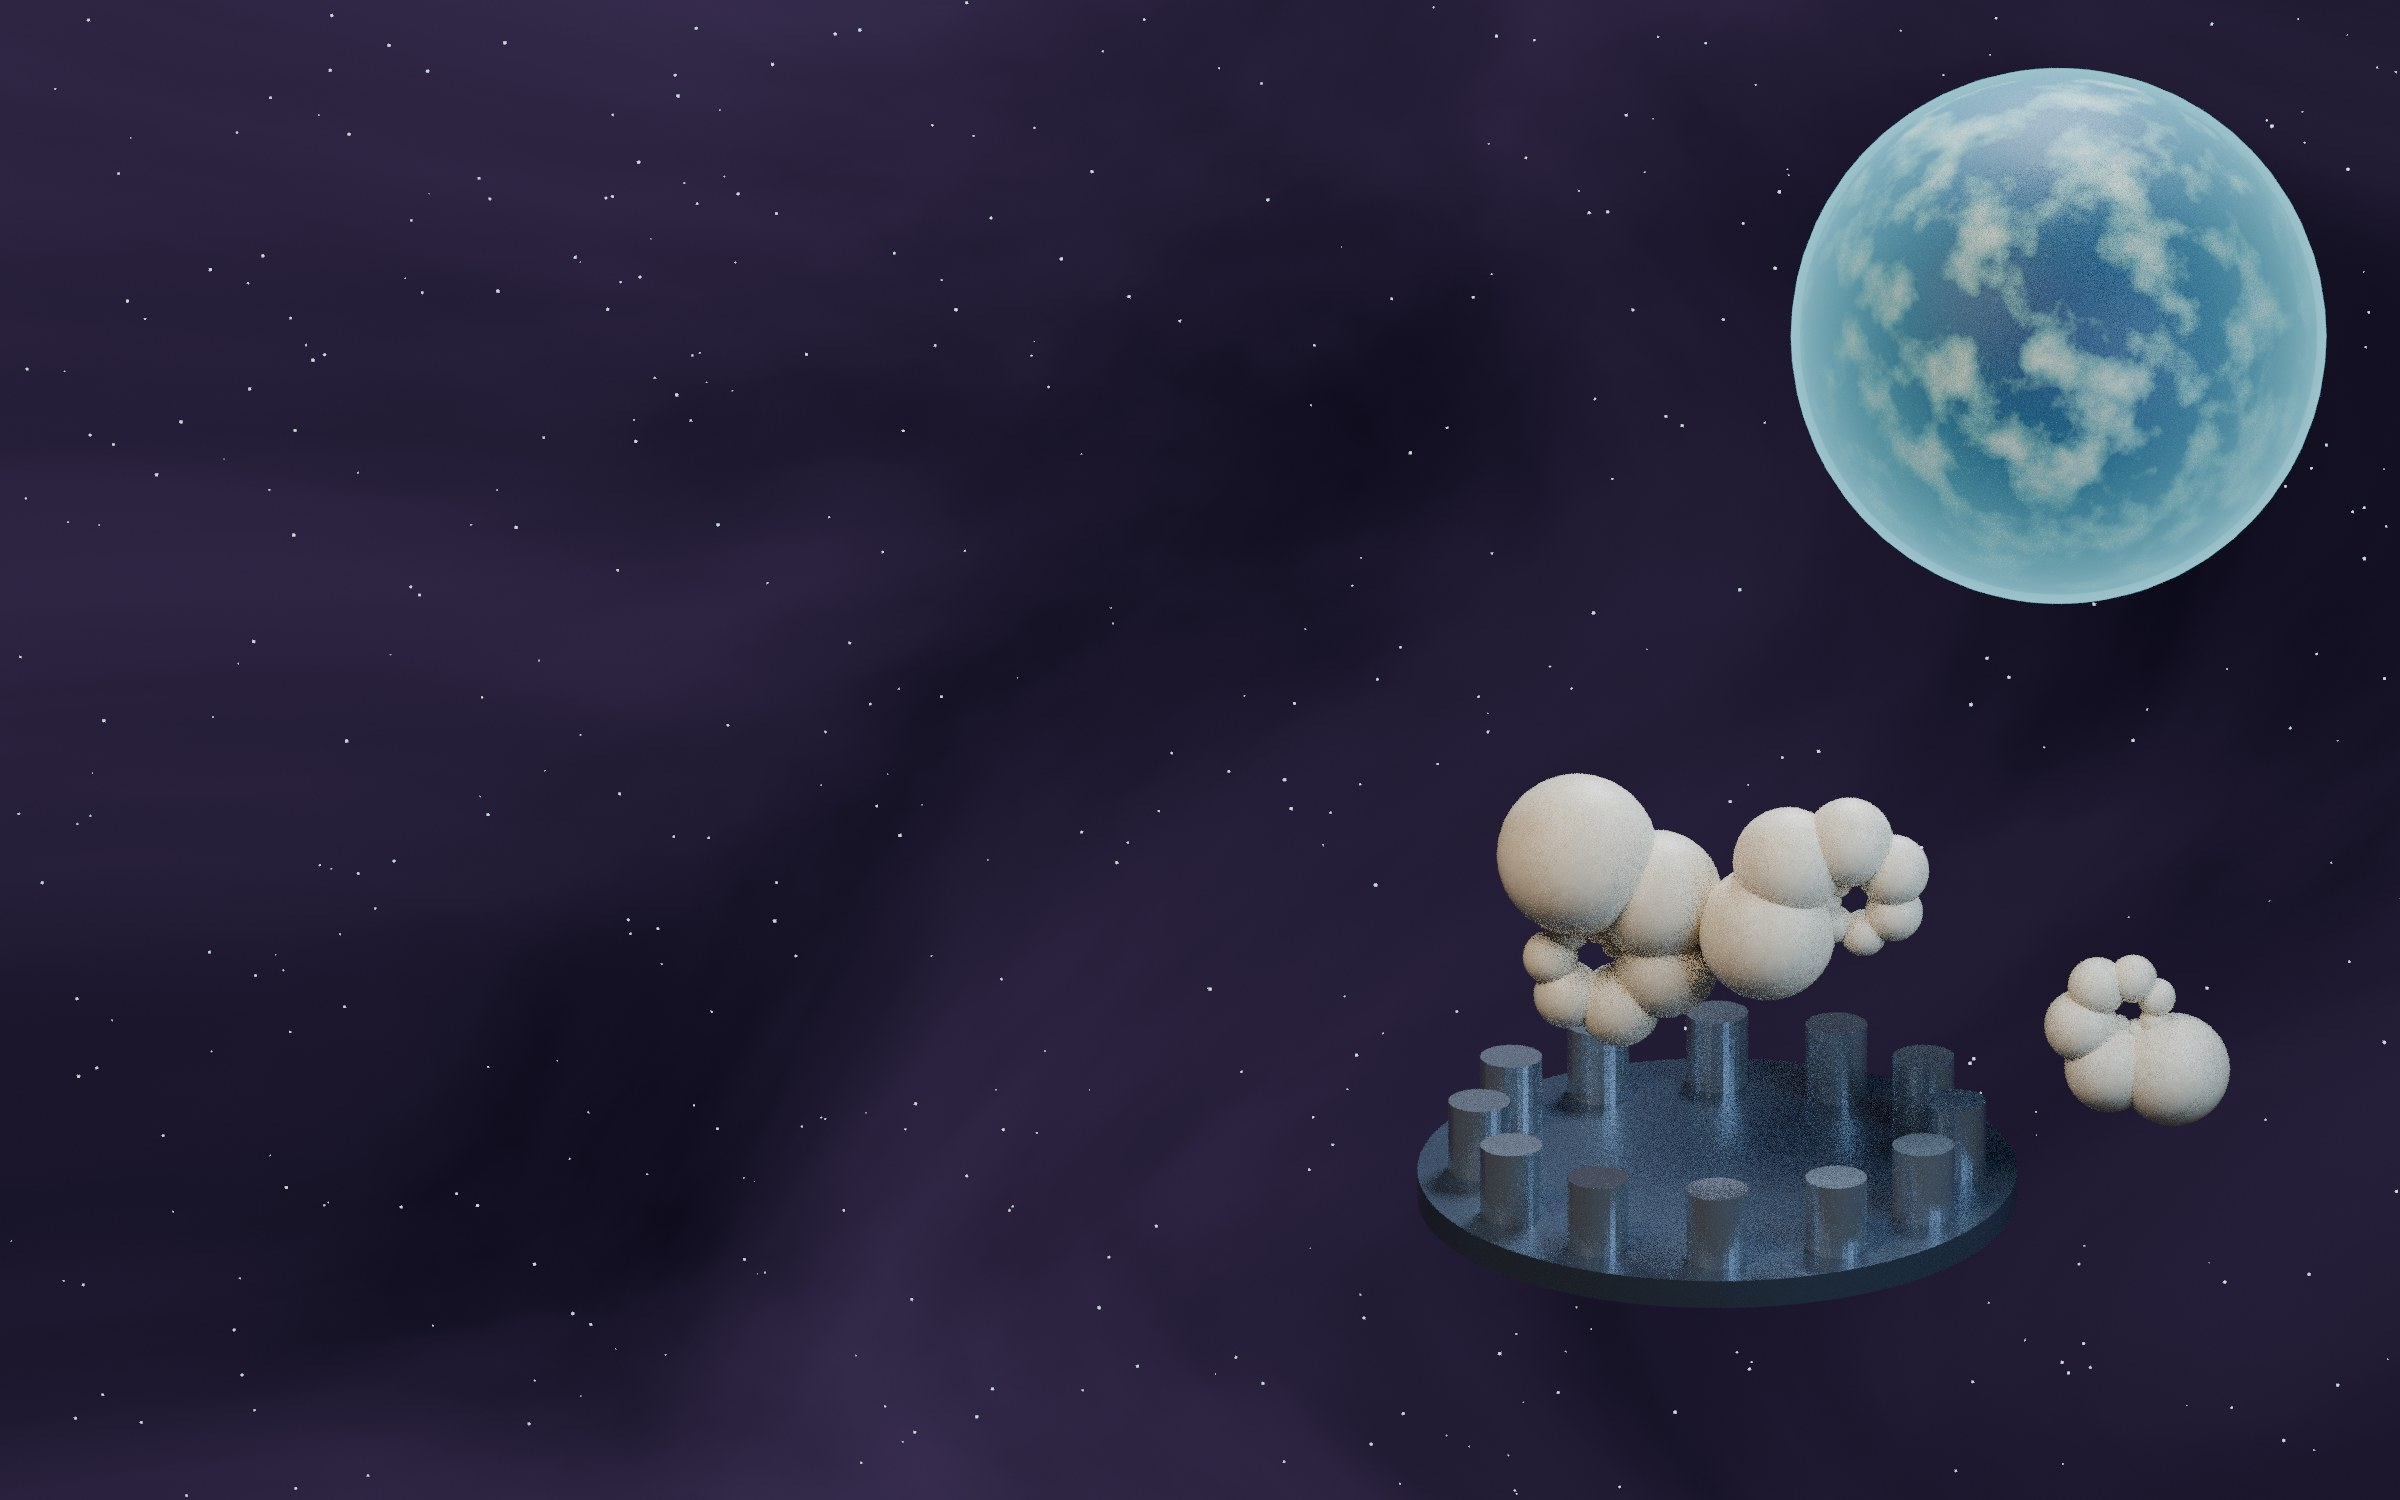
\includegraphics[width=20cm,height=12.5cm]{Scena/copertina.jpg}};}{}
\node[anchor=north west,inner sep=0] at([xshift=1.05cm,yshift=-1.10cm]current page.north west){\color{Mint}\bfseries\fontsize{23}{28}\selectfont SPEDIZIONE P02};
\node[anchor=north west,inner sep=0] at([xshift=1.07cm,yshift=-2.16cm]current page.north west){\color{white}\fontsize{9}{12}\selectfont MACROPROGETTO P02 · SCIENZE DELLA TERRA};
\draw[Mint,line width=1.5pt]([xshift=1.07cm,yshift=-2.78cm]current page.north west)--([xshift=2.6cm,yshift=-2.78cm]current page.north west);
\node[anchor=north west,inner sep=0] at([xshift=1.05cm,yshift=-3.35cm]current page.north west){\begin{minipage}{9.2cm}\raggedright\color{white}\bfseries\fontsize{28.5}{34.5}\selectfont Foraminiferi,\\coppe e campagne\end{minipage}};
\node[anchor=north west,inner sep=0] at([xshift=1.07cm,yshift=-7.88cm]current page.north west){\begin{minipage}{8.9cm}\raggedright\color{Lilac}\fontsize{12.2}{17}\selectfont Trentasei coppe, quattro campagne appaiate\end{minipage}};
\node[anchor=north west,inner sep=0] at([xshift=1.07cm,yshift=-8.70cm]current page.north west){\begin{minipage}{8.9cm}\raggedright\color{white!75}\fontsize{10.3}{14.5}\selectfont Copertura temporale, confronti appaiati e limiti di quattro repliche\end{minipage}};
\node[anchor=north west,inner sep=0] at([xshift=1.07cm,yshift=-10.52cm]current page.north west){\color{white}\fontsize{10.5}{14}\selectfont GeoStat Lab · corso di Marzio De Corato};
\node[anchor=north west,inner sep=0] at([xshift=1.07cm,yshift=-11.17cm]current page.north west){\color{Mint}\fontsize{8.8}{11}\selectfont\href{https://creativecommons.org/licenses/by-nc-sa/4.0/}{Impaginazione da Tessera · CC BY-NC-SA 4.0}};
\end{tikzpicture}\end{frame}

\begin{frame}[plain]\hypertarget{slide2}{}
\bookmark[level=1,page=2]{Indice della presentazione}
\begin{tikzpicture}[remember picture,overlay]
\PilotChrome{Indice della presentazione}{PERCORSO}{2}{I titoli dell’indice aprono i capitoli. Il nome del capitolo in alto riporta a questa pagina.}
\node[anchor=north west,inner sep=0] at([xshift=.96cm,yshift=-2.12cm]current page.north west){\Colonna{9.40cm}{\PLabel{Capitoli}
{\fontsize{10.7}{13.5}\selectfont\hyperlink{slide4}{Fonte e supporto delle osservazioni\hfill 4}\par}\vspace{.16cm}
{\fontsize{10.7}{13.5}\selectfont\hyperlink{slide7}{Copertura e definizione del confronto\hfill 7}\par}\vspace{.16cm}
{\fontsize{10.7}{13.5}\selectfont\hyperlink{slide15}{Incertezza con quattro unità\hfill 15}\par}\vspace{.16cm}
{\fontsize{10.7}{13.5}\selectfont\hyperlink{slide21}{Interpretazione e nuova raccolta\hfill 21}\par}\vspace{.16cm}
{\fontsize{10.7}{13.5}\selectfont\hyperlink{slide24}{Laboratori della spedizione\hfill 24}\par}\vspace{.16cm}

}};
\node[anchor=north west,inner sep=0] at([xshift=10.85cm,yshift=-2.12cm]current page.north west){\Colonna{8.16cm}{\PLabel{Percorso di lettura}
\PBody{Il percorso esamina la fonte e la copertura delle campagne, definisce il confronto appaiato, ne misura l’incertezza con quattro unità e prepara una nuova raccolta. I laboratori finali riprendono le tre fasi della spedizione.}
\PInfo{Le pagine Scenario A e Confronto riprendono gli esperimenti nel browser con dati sintetici. I valori di partenza del simulatore differiscono da quelli del caso.}
\href{https://marzione00.github.io/Lab_Geo/\#modulo-P02}{\color{Classical}\bfseries Apri la spedizione P02 su GeoStat Lab}
}};
\end{tikzpicture}\end{frame}

\begin{frame}[plain]\hypertarget{slide3}{}
\bookmark[level=1,page=3]{La taglia di Neogloboquadrina pachyderma cambia fra le fasce ottobre–marzo e aprile–settembre?}
\begin{tikzpicture}[remember picture,overlay]
\PilotChrome{{\fontsize{15.3}{19}\selectfont La taglia di Neogloboquadrina pachyderma cambia fra le fasce ottobre–marzo e aprile–settembre?}}{IL CASO GUIDA}{3}{La copertina è una scena illustrativa. Le misure provengono dall’estratto PANGAEA del supplemento di Mikis e collaboratori.}
\node[anchor=north west,inner sep=0] at([xshift=.96cm,yshift=-2.12cm]current page.north west){\Colonna{9.40cm}{{\centering\resizebox{0.97\linewidth}{!}{\begin{tikzpicture}[x=1cm,y=1cm,every node/.style={font=\sffamily\fontsize{10}{12}\selectfont,text=Ink}]
\draw[draw=Classical,fill=Classical!8,rounded corners=2mm,line width=.7pt] (0,0.00) rectangle (8.6,-0.78);
\node[circle,anchor=center,fill=Classical,inner sep=0,minimum size=.5cm,text=white,font=\sffamily\bfseries\fontsize{9}{10}\selectfont] at (.48,-0.39) {1};
\node[anchor=west,text width=7.4cm,align=left] at (.95,-0.39) {Fonte e supporto delle osservazioni};
\draw[pEdge] (.48,-0.80)--(.48,-1.02);
\draw[draw=Classical,fill=Classical!8,rounded corners=2mm,line width=.7pt] (0,-1.04) rectangle (8.6,-1.82);
\node[circle,anchor=center,fill=Classical,inner sep=0,minimum size=.5cm,text=white,font=\sffamily\bfseries\fontsize{9}{10}\selectfont] at (.48,-1.43) {2};
\node[anchor=west,text width=7.4cm,align=left] at (.95,-1.43) {Copertura e definizione del confronto};
\draw[pEdge] (.48,-1.84)--(.48,-2.06);
\draw[draw=Classical,fill=Classical!8,rounded corners=2mm,line width=.7pt] (0,-2.08) rectangle (8.6,-2.86);
\node[circle,anchor=center,fill=Classical,inner sep=0,minimum size=.5cm,text=white,font=\sffamily\bfseries\fontsize{9}{10}\selectfont] at (.48,-2.47) {3};
\node[anchor=west,text width=7.4cm,align=left] at (.95,-2.47) {Incertezza con quattro unità};
\draw[pEdge] (.48,-2.88)--(.48,-3.10);
\draw[draw=Classical,fill=Classical!8,rounded corners=2mm,line width=.7pt] (0,-3.12) rectangle (8.6,-3.90);
\node[circle,anchor=center,fill=Classical,inner sep=0,minimum size=.5cm,text=white,font=\sffamily\bfseries\fontsize{9}{10}\selectfont] at (.48,-3.51) {4};
\node[anchor=west,text width=7.4cm,align=left] at (.95,-3.51) {Interpretazione e nuova raccolta};
\draw[pEdge] (.48,-3.92)--(.48,-4.14);
\draw[draw=GeoB,fill=GeoB!8,rounded corners=2mm,line width=.7pt] (0,-4.16) rectangle (8.6,-4.94);
\node[circle,anchor=center,fill=GeoB,inner sep=0,minimum size=.5cm,text=white,font=\sffamily\bfseries\fontsize{9}{10}\selectfont] at (.48,-4.55) {L};
\node[anchor=west,text width=7.4cm,align=left] at (.95,-4.55) {Laboratori della spedizione};
\end{tikzpicture}
}\par}
\PSmall{Capitoli della spedizione; L indica i laboratori conclusivi.}
}};
\node[anchor=north west,inner sep=0] at([xshift=10.85cm,yshift=-2.12cm]current page.north west){\Colonna{8.16cm}{\PLabel{Il caso}
\PBody{Trentasei coppe di una trappola sedimentaria della Penisola Antartica occidentale, a 170 metri di profondità, registrano il diametro medio di N. pachyderma in sei campagne. Soltanto quattro campagne coprono entrambe le fasce calendario.}
\PInfo{Seguiremo il passaggio dalle coppe riunite alle differenze di campagna, con intervallo t, bootstrap, ribaltamento dei segni e sensibilità alla singola campagna.}
}};
\end{tikzpicture}\end{frame}

\begin{frame}[plain]\hypertarget{slide4}{}
\bookmark[level=0,page=4]{Fonte e supporto delle osservazioni}
\bookmark[level=1,page=4]{Una domanda sulla variazione della taglia}
\begin{tikzpicture}[remember picture,overlay]
\PilotChrome{Una domanda sulla variazione della taglia}{FONTE E SUPPORTO DELLE OSSERVAZIONI}{4}{La domanda deve rispettare il supporto temporale e materiale della misura disponibile.}
\node[anchor=north west,inner sep=0] at([xshift=.96cm,yshift=-2.12cm]current page.north west){\Colonna{9.40cm}{{\centering\resizebox{0.90\linewidth}{!}{\begin{tikzpicture}[x=1cm,y=-.87cm,every node/.style={font=\fontsize{12.2}{15}\selectfont,text=Ink},arr/.style={-{Stealth[length=2mm]},line width=.8pt,draw=Classical}]\path[use as bounding box] (0,0) rectangle (7.45,6.2);
\draw[Quantum,line width=.8pt] (0.6,0.7)--(6.8,0.7);
\node[anchor=center,text=Ink,font=\fontsize{11}{15}\selectfont,text width=6cm,align=center] at (3.7,0.25) {Superficie marina};
\draw[Classical,fill=Classical!8,line width=.8pt] (2,2)--(5.4,2)--(4.1,3.4)--(3.3,3.4)--cycle;\draw[draw=Classical,fill=Classical!8,rounded corners=2pt,line width=.7pt] (3.1,3.6) rectangle (4.3,4.7);
\node[anchor=center,text=Ink,font=\fontsize{11.5}{15}\selectfont,text width=6.6cm,align=center] at (3.7,5.25) {Raccolta integrata nel tempo};
\draw[arr,draw=Quantum] (1.2,1.1)--(1.2,3.4);
\node[anchor=center,text=Ink,font=\fontsize{11}{15}\selectfont,text width=1.9cm,align=center] at (1.2,4.2) {170 m};
\node[anchor=center,text=Ink,font=\fontsize{10.5}{15}\selectfont,text width=6.8cm,align=center] at (3.7,6) {Schema non in scala.};

\end{tikzpicture}}\par}
}};
\node[anchor=north west,inner sep=0] at([xshift=10.85cm,yshift=-2.12cm]current page.north west){\Colonna{8.16cm}{\PBody{Il progetto esamina il diametro massimo medio di Neogloboquadrina pachyderma in coppe di una trappola sedimentaria della Penisola Antartica occidentale, collocata a 170 metri di profondità. L’estratto PANGAEA conserva trentasei righe del supplemento di Mikis e collaboratori, con date centrali e sintesi morfometriche. La domanda confronta le fasce calendario ottobre–marzo e aprile–settembre nelle campagne che le rappresentano entrambe. Le fasce definiscono un criterio temporale di raggruppamento, del quale occorre distinguere il significato dalle condizioni ambientali effettivamente vissute dagli organismi.}
}};
\end{tikzpicture}\end{frame}

\begin{frame}[plain]\hypertarget{slide5}{}
\bookmark[level=1,page=5]{La riga rappresenta una sintesi di coppa}
\begin{tikzpicture}[remember picture,overlay]
\PilotChrome{La riga rappresenta una sintesi di coppa}{FONTE E SUPPORTO DELLE OSSERVAZIONI}{5}{Il livello di aggregazione della fonte determina quali quantità siano identificabili dai dati.}
\node[anchor=north west,inner sep=0] at([xshift=.96cm,yshift=-2.12cm]current page.north west){\Colonna{9.40cm}{{\centering\resizebox{0.90\linewidth}{!}{\begin{tikzpicture}[x=1cm,y=-.87cm,every node/.style={font=\fontsize{12.2}{15}\selectfont,text=Ink},arr/.style={-{Stealth[length=2mm]},line width=.8pt,draw=Classical}]\path[use as bounding box] (0,0) rectangle (7.45,6.2);
\draw[draw=Classical,fill=Classical!8,rounded corners=2pt,line width=.7pt] (0.5,0.6) rectangle (6.9,1.9);
\node[anchor=center,text=Ink,font=\fontsize{12.2}{15}\selectfont,text width=6cm,align=center] at (3.7,1.25) {Individui analizzati nella coppa};
\draw[arr,draw=Classical] (3.7,2.1)--(3.7,2.7);
\draw[draw=Quantum,fill=Quantum!8,rounded corners=2pt,line width=.7pt] (0.5,2.9) rectangle (6.9,4.2);
\node[anchor=center,text=Ink,font=\fontsize{11.5}{15}\selectfont,text width=6cm,align=center] at (3.7,3.55) {Media, mediana ed estremi pubblicati};
\node[anchor=center,text=Ink,font=\fontsize{12.2}{15}\selectfont,text width=6.7cm,align=center] at (3.7,5.4) {Una riga conserva una sintesi già eseguita.};

\end{tikzpicture}}\par}
}};
\node[anchor=north west,inner sep=0] at([xshift=10.85cm,yshift=-2.12cm]current page.north west){\Colonna{8.16cm}{\PBody{Ogni riga contiene una sintesi degli individui analizzati nella coppa, con media, mediana, minimo e massimo del diametro massimo. La tabella selezionata non include il numero degli individui né la loro deviazione standard, per cui queste quantità non possono essere ricostruite a partire dai soli estremi. Il confronto usa medie di coppa e mantiene esplicita questa unità. Aumentare il numero di gusci misurati entro una coppa e aumentare il numero di campagne indipendenti migliorerebbe componenti differenti dell’informazione.}
}};
\end{tikzpicture}\end{frame}

\begin{frame}[plain]\hypertarget{slide6}{}
\bookmark[level=1,page=6]{Controlli sul dizionario e sulle sintesi}
\begin{tikzpicture}[remember picture,overlay]
\PilotChrome{Controlli sul dizionario e sulle sintesi}{FONTE E SUPPORTO DELLE OSSERVAZIONI}{6}{La plausibilità delle sintesi non sostituisce le informazioni sul protocollo e sul numero degli individui.}
\node[anchor=north west,inner sep=0] at([xshift=.96cm,yshift=-2.12cm]current page.north west){\Colonna{9.40cm}{\PBody{La coppia campagna–coppa identifica ogni riga e viene verificata prima del raggruppamento. Il codice controlla profondità, conversione delle date e ordine fra minimo, media e massimo, mantenendo le unità in micrometri. Gli estremi descrivono la dispersione degli individui osservati e non costituiscono un intervallo di confidenza della media. La data rappresenta il punto centrale attribuito alla coppa; la durata della raccolta e il flusso di gusci richiederebbero metadati ulteriori per una ponderazione temporale o quantitativa.}
}};
\node[anchor=north west,inner sep=0] at([xshift=10.85cm,yshift=-2.12cm]current page.north west){\Colonna{8.16cm}{\begin{tcolorbox}[enhanced,arc=1.7mm,boxrule=.6pt,colback=white,colframe=Classical!60!Navy,colbacktitle=Navy,coltitle=white,fonttitle=\bfseries\small,title={R · calcolo riproducibile},left=1.7mm,right=1.3mm,top=1.1mm,bottom=1.1mm,before skip=1mm,after skip=1.0mm]\lstinputlisting[style=GeoR,language=R,basicstyle=\ttfamily\fontsize{8.6}{11.4}\selectfont]{Codice/audit.R}\end{tcolorbox}
\PLabel{Risultato in R}
\begin{tcolorbox}[colback=GeoTint,colframe=Rule,boxrule=.5pt,arc=1.4mm,left=2mm,right=1mm,top=1mm,bottom=1mm]{\fontsize{8.4}{10.9}\selectfont\ttfamily \mbox{\ \ \ Min.\ 1st\ Qu.\ \ Median\ \ \ \ Mean\ 3rd\ Qu.\ \ \ \ Max.\ }\\\mbox{\ \ 171.4\ \ \ 222.5\ \ \ 248.3\ \ \ 249.5\ \ \ 279.1\ \ \ 325.3\ }}\end{tcolorbox}
}};
\end{tikzpicture}\end{frame}

\begin{frame}[plain]\hypertarget{slide7}{}
\bookmark[level=0,page=7]{Copertura e definizione del confronto}
\bookmark[level=1,page=7]{Due fasce calendario definite prima del calcolo}
\begin{tikzpicture}[remember picture,overlay]
\PilotChrome{Due fasce calendario definite prima del calcolo}{COPERTURA E DEFINIZIONE DEL CONFRONTO}{7}{La regola temporale definisce il confronto e mantiene distinti calendario e processo ambientale.}
\node[anchor=north west,inner sep=0] at([xshift=.96cm,yshift=-2.12cm]current page.north west){\Colonna{9.40cm}{\PBody{La classificazione assegna ottobre, novembre, dicembre, gennaio, febbraio e marzo alla prima fascia, lasciando aprile–settembre alla seconda. Il mese viene ricavato dalla data centrale della coppa e la campagna mantiene l’identificativo fornito nella fonte. La regola è riproducibile e lascia fuori dalla misura temperatura, luce, alimento e condizioni di dissoluzione. La denominazione delle fasce conserva pertanto i mesi effettivi, evitando di trasformare il raggruppamento in una diagnosi automatica del meccanismo stagionale.}
\par\smallskip{\centering\adjustbox{max width=.98\linewidth}{$\displaystyle \begin{gathered}S_i=\begin{cases}1,&m_i\in\{10{,}11{,}12{,}1{,}2{,}3\},\\0,&m_i\in\{4{,}5{,}6{,}7{,}8{,}9\}.\end{cases}\end{gathered}$}\par\smallskip}
}};
\node[anchor=north west,inner sep=0] at([xshift=10.85cm,yshift=-2.12cm]current page.north west){\Colonna{8.16cm}{\PInfo{$m_i$: mese della data centrale della coppa i; $S_i$: indicatore della fascia ottobre–marzo. Una diversa definizione modificherebbe il confronto e andrebbe giustificata prima dell’esito. Per coppe che attraversano il confine, la data centrale è una convenzione, la cui sensibilità può essere studiata con le date di apertura e chiusura.}
}};
\end{tikzpicture}\end{frame}

\begin{frame}[plain]\hypertarget{slide8}{}
\bookmark[level=1,page=8]{L’irregolarità temporale resta visibile}
\begin{tikzpicture}[remember picture,overlay]
\PilotChrome{L’irregolarità temporale resta visibile}{COPERTURA E DEFINIZIONE DEL CONFRONTO}{8}{La rappresentazione temporale rende riconoscibile il supporto osservativo del confronto.}
\node[anchor=north west,inner sep=0] at([xshift=.96cm,yshift=-2.12cm]current page.north west){\Colonna{9.40cm}{{\centering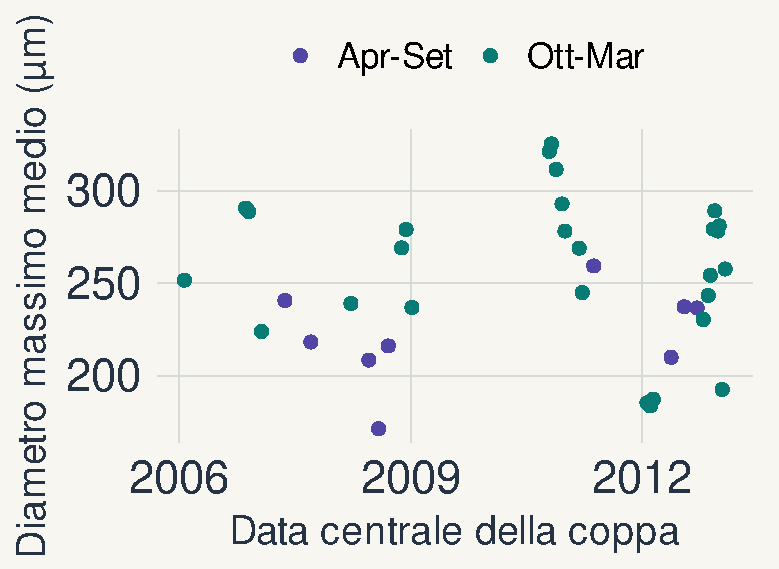
\includegraphics[width=\linewidth,height=6.15cm,keepaspectratio]{Figure/F01.pdf}\par}
\PSmall{Trentasei medie di coppa, rappresentate alle date centrali. Le interruzioni della serie rimangono esplicite.}
}};
\node[anchor=north west,inner sep=0] at([xshift=10.85cm,yshift=-2.12cm]current page.north west){\Colonna{8.16cm}{\PBody{Le trentasei medie sono rappresentate alle rispettive date centrali senza unirle mediante una linea continua. Questa scelta conserva le lacune e la diversa densità di campionamento, evitando che il disegno suggerisca valori nei periodi privi di osservazioni. I colori distinguono le due fasce calendario, mentre la variabilità dei punti riflette insieme differenze fra coppe, campagne e condizioni di raccolta. La figura precede ogni test perché rende evidente che la composizione dei gruppi dipende dalla copertura disponibile.}
}};
\end{tikzpicture}\end{frame}

\begin{frame}[plain]\hypertarget{slide9}{}
\bookmark[level=1,page=9]{La matrice dei conteggi identifica le coppie}
\begin{tikzpicture}[remember picture,overlay]
\PilotChrome{La matrice dei conteggi identifica le coppie}{COPERTURA E DEFINIZIONE DEL CONFRONTO}{9}{La copertura determina quali confronti siano sostenuti dai dati e con quali pesi.}
\node[anchor=north west,inner sep=0] at([xshift=.96cm,yshift=-2.12cm]current page.north west){\Colonna{9.40cm}{{\centering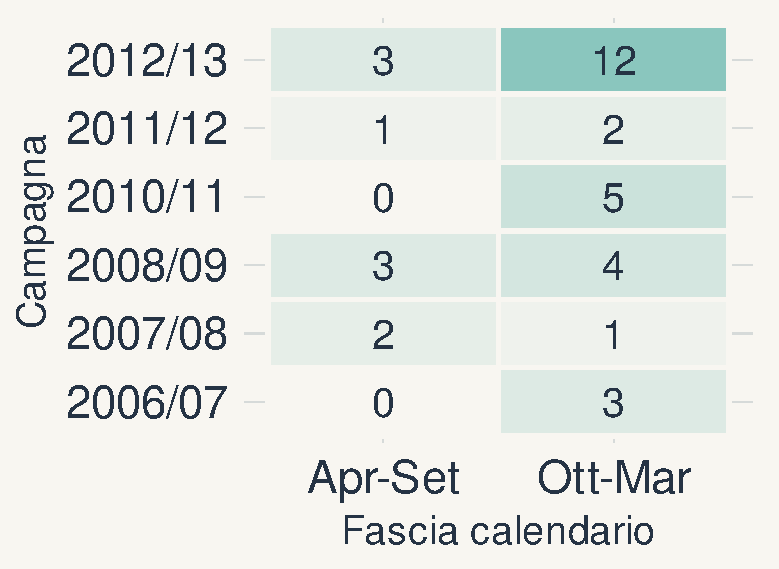
\includegraphics[width=\linewidth,height=6.15cm,keepaspectratio]{Figure/F02.pdf}\par}
\PSmall{Numero di coppe per campagna e fascia. Una cella vuota di osservazioni è indicata da zero.}
}};
\node[anchor=north west,inner sep=0] at([xshift=10.85cm,yshift=-2.12cm]current page.north west){\Colonna{8.16cm}{\PBody{La tabella grafica incrocia le sei campagne con le due fasce e riporta il numero di coppe disponibili in ogni cella. Due campagne rappresentano soltanto una fascia, mentre quattro contengono entrambe le condizioni necessarie al confronto appaiato. I conteggi differiscono anche nelle campagne complete, per cui una media su tutte le coppe attribuirebbe pesi disuguali agli anni. La selezione delle campagne complete definisce una popolazione osservativa più ristretta, della quale devono essere dichiarate composizione e ragione dell’inclusione.}
}};
\end{tikzpicture}\end{frame}

\begin{frame}[plain]\hypertarget{slide10}{}
\bookmark[level=1,page=10]{Media delle coppe riunite e pesi impliciti}
\begin{tikzpicture}[remember picture,overlay]
\PilotChrome{Media delle coppe riunite e pesi impliciti}{COPERTURA E DEFINIZIONE DEL CONFRONTO}{10}{Una probabilità piccola non corregge una scelta inadeguata dell’unità o della ponderazione.}
\node[anchor=north west,inner sep=0] at([xshift=.96cm,yshift=-2.12cm]current page.north west){\Colonna{9.40cm}{\PBody{Riunendo tutte le coppe di ciascuna fascia, la differenza risulta circa 36,66 micrometri. Il confronto Welch restituisce una probabilità di riferimento prossima a 0,004, assumendo indipendenza fra coppe e ignorando la struttura delle campagne. Questo controesempio attribuisce maggiore peso alle campagne più campionate, includendo quelle incomplete soltanto in una fascia. La quantità stimata e il modello di dipendenza differiscono quindi da quelli del confronto per campagne complete.}
\par\smallskip{\centering\adjustbox{max width=.98\linewidth}{$\displaystyle \widehat\Delta_{coppe}=\frac1{N_1}\sum_{i:S_i=1}y_i-\frac1{N_0}\sum_{i:S_i=0}y_i$}\par\smallskip}
}};
\node[anchor=north west,inner sep=0] at([xshift=10.85cm,yshift=-2.12cm]current page.north west){\Colonna{8.16cm}{\PInfo{$y_i$: diametro massimo medio della coppa i, in µm; $S_i=1$: ottobre–marzo, $S_i=0$: aprile–settembre. $N_s$ conta le coppe nella fascia s. La differenza rispetto alla stima appaiata riflette composizione e ponderazione: cambia anche l’oggetto della media, oltre alla formula dell’errore standard.}
}};
\end{tikzpicture}\end{frame}

\begin{frame}[plain]\hypertarget{slide11}{}
\bookmark[level=1,page=11]{L’estimando delle campagne complete}
\begin{tikzpicture}[remember picture,overlay]
\PilotChrome{L’estimando delle campagne complete}{COPERTURA E DEFINIZIONE DEL CONFRONTO}{11}{Il denominatore finale è costituito dalle quattro campagne complete.}
\node[anchor=north west,inner sep=0] at([xshift=.96cm,yshift=-2.12cm]current page.north west){\Colonna{9.40cm}{{\centering\resizebox{0.90\linewidth}{!}{\begin{tikzpicture}[x=1cm,y=-.87cm,every node/.style={font=\fontsize{12.2}{15}\selectfont,text=Ink},arr/.style={-{Stealth[length=2mm]},line width=.8pt,draw=Classical}]\path[use as bounding box] (0,0) rectangle (7.45,6.2);
\draw[draw=Classical,fill=Classical!8,rounded corners=2pt,line width=.7pt] (0.5,0.5) rectangle (6.9,1.8);
\node[anchor=center,text=Ink,font=\fontsize{11.5}{15}\selectfont,text width=6cm,align=center] at (3.7,1.15) {Media delle coppe entro fascia e campagna};
\draw[arr,draw=Classical] (3.7,2)--(3.7,2.6);
\draw[draw=Quantum,fill=Quantum!8,rounded corners=2pt,line width=.7pt] (0.5,2.8) rectangle (6.9,4.1);
\node[anchor=center,text=Ink,font=\fontsize{11.5}{15}\selectfont,text width=6cm,align=center] at (3.7,3.45) {Una differenza per campagna completa};
\draw[arr,draw=Classical] (3.7,4.3)--(3.7,4.9);
\node[anchor=center,text=Ink,font=\fontsize{11.5}{15}\selectfont,text width=6.7cm,align=center] at (3.7,5.5) {Media di quattro differenze equiponderate};

\end{tikzpicture}}\par}
\PSmall{g: campagna; s: fascia, 1 per ottobre–marzo e 0 per aprile–settembre. $n_{gs}$: coppe disponibili; $y_i$: media della coppa, in µm.}
}};
\node[anchor=north west,inner sep=0] at([xshift=10.85cm,yshift=-2.12cm]current page.north west){\Colonna{8.16cm}{\PBody{Si calcola la media delle coppe entro ogni combinazione campagna–fascia e poi la differenza ottobre–marzo meno aprile–settembre. La media finale assegna uguale peso alle quattro campagne complete, indipendentemente dal numero delle coppe. Una ponderazione per durata, individui o flusso sedimentario definirebbe un’altra quantità, che richiederebbe informazioni ulteriori.}
\par\smallskip{\centering\adjustbox{max width=.98\linewidth}{$\displaystyle \begin{gathered}\overline y_{gs}=\frac1{n_{gs}}\sum_{i\in(g,s)}y_i,\qquad d_g=\overline y_{g1}-\overline y_{g0}\\\widehat\Delta=\frac14\sum_{g=1}^{4}d_g\end{gathered}$}\par\smallskip}
}};
\end{tikzpicture}\end{frame}

\begin{frame}[plain]\hypertarget{slide12}{}
\bookmark[level=1,page=12]{Costruzione delle coppie in R}
\begin{tikzpicture}[remember picture,overlay]
\PilotChrome{Costruzione delle coppie in R}{COPERTURA E DEFINIZIONE DEL CONFRONTO}{12}{La trasformazione della tabella deve conservare la corrispondenza fra le due medie della medesima campagna.}
\node[anchor=north west,inner sep=0] at([xshift=.96cm,yshift=-2.12cm]current page.north west){\Colonna{9.40cm}{\PBody{Il raggruppamento produce una riga per campagna e fascia, mentre la trasformazione in formato largo colloca le due medie sulla stessa riga. La selezione delle righe complete rende esplicito il requisito dell’appaiamento. Le etichette S1 e S0 indicano rispettivamente ottobre–marzo e aprile–settembre. Il controllo di quattro differenze e il confronto con la tabella esportata permettono di verificare che la costruzione delle coppie rispetti il protocollo dichiarato.}
}};
\node[anchor=north west,inner sep=0] at([xshift=10.85cm,yshift=-2.12cm]current page.north west){\Colonna{8.16cm}{\begin{tcolorbox}[enhanced,arc=1.7mm,boxrule=.6pt,colback=white,colframe=Classical!60!Navy,colbacktitle=Navy,coltitle=white,fonttitle=\bfseries\small,title={R · calcolo riproducibile},left=1.7mm,right=1.3mm,top=1.1mm,bottom=1.1mm,before skip=1mm,after skip=1.0mm]\lstinputlisting[style=GeoR,language=R,basicstyle=\ttfamily\fontsize{8.6}{11.4}\selectfont]{Codice/coppie.R}\end{tcolorbox}
\PLabel{Risultato in R}
\begin{tcolorbox}[colback=GeoTint,colframe=Rule,boxrule=.5pt,arc=1.4mm,left=2mm,right=1mm,top=1mm,bottom=1mm]{\fontsize{8.4}{10.9}\selectfont\ttfamily \mbox{[1]\ 14.99083}}\end{tcolorbox}
}};
\end{tikzpicture}\end{frame}

\begin{frame}[plain]\hypertarget{slide13}{}
\bookmark[level=1,page=13]{Le quattro coppie mostrano andamenti differenti}
\begin{tikzpicture}[remember picture,overlay]
\PilotChrome{Le quattro coppie mostrano andamenti differenti}{COPERTURA E DEFINIZIONE DEL CONFRONTO}{13}{La struttura appaiata rende visibile la variabilità delle differenze che entrano nell’inferenza.}
\node[anchor=north west,inner sep=0] at([xshift=.96cm,yshift=-2.12cm]current page.north west){\Colonna{9.40cm}{{\centering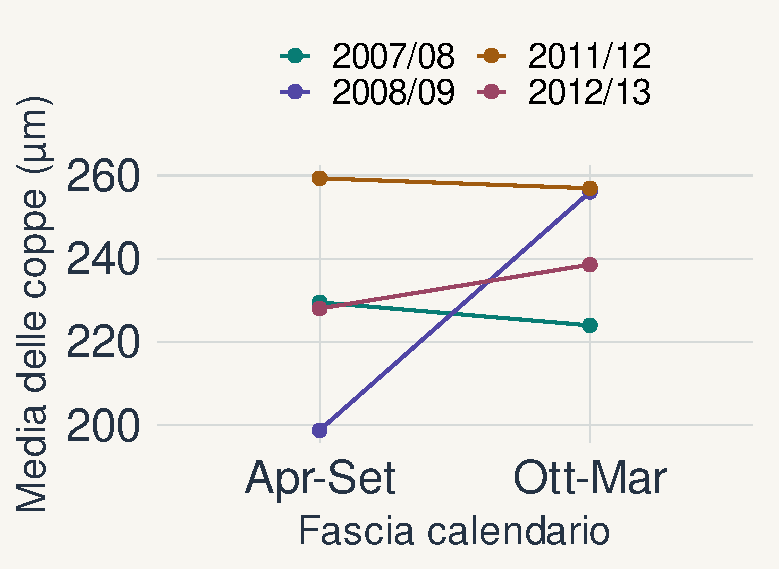
\includegraphics[width=\linewidth,height=6.15cm,keepaspectratio]{Figure/F03.pdf}\par}
\PSmall{Medie delle coppe nelle quattro campagne complete. Ogni linea collega le due fasce della stessa campagna.}
}};
\node[anchor=north west,inner sep=0] at([xshift=10.85cm,yshift=-2.12cm]current page.north west){\Colonna{8.16cm}{\PBody{Le linee collegano le due medie della stessa campagna e rendono visibile l’eterogeneità dei confronti. Due campagne mostrano differenze negative, una una differenza positiva contenuta e una un incremento molto maggiore. Le linee descrivono un abbinamento fra medie di fascia, senza rappresentare una traiettoria continua nel tempo. Il grafico suggerisce di studiare direttamente le quattro differenze, poiché una sintesi complessiva potrebbe nascondere il contributo sproporzionato di una singola campagna.}
}};
\end{tikzpicture}\end{frame}

\begin{frame}[plain]\hypertarget{slide14}{}
\bookmark[level=1,page=14]{Quattro differenze come osservazioni dell’analisi}
\begin{tikzpicture}[remember picture,overlay]
\PilotChrome{Quattro differenze come osservazioni dell’analisi}{COPERTURA E DEFINIZIONE DEL CONFRONTO}{14}{Segno, grandezza e variabilità delle differenze precedono l’interpretazione del test.}
\node[anchor=north west,inner sep=0] at([xshift=.96cm,yshift=-2.12cm]current page.north west){\Colonna{9.40cm}{{\centering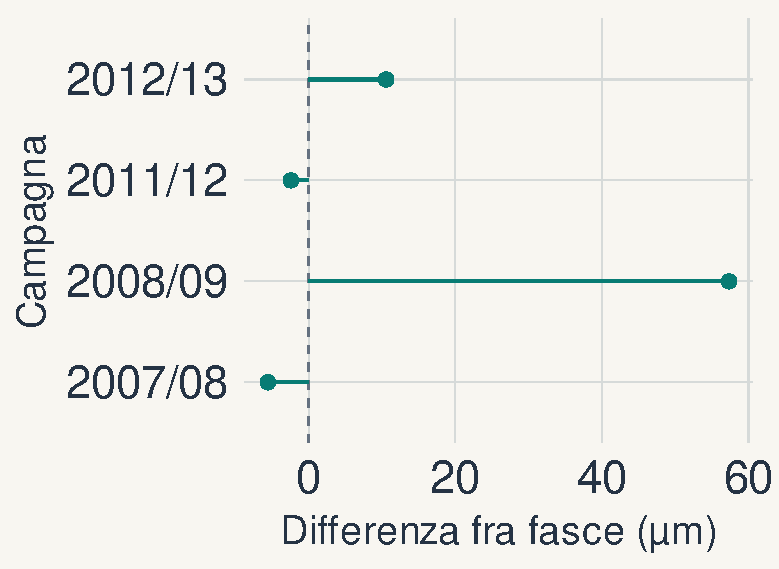
\includegraphics[width=\linewidth,height=6.15cm,keepaspectratio]{Figure/F04.pdf}\par}
\PSmall{Differenza ottobre–marzo meno aprile–settembre. La linea verticale indica uguaglianza fra le due medie di fascia.}
}};
\node[anchor=north west,inner sep=0] at([xshift=10.85cm,yshift=-2.12cm]current page.north west){\Colonna{8.16cm}{\PBody{Le differenze sono circa meno 5,55, più 57,35, meno 2,41 e più 10,57 micrometri, nelle quattro campagne ordinate cronologicamente. La loro media è circa 14,99 micrometri, mentre la dispersione rimane elevata rispetto a questa grandezza. La campagna 2008–2009 contribuisce in modo rilevante alla media positiva. I valori disponibili descrivono campagne di uno stesso sito e non garantiscono indipendenza temporale; tale ipotesi va discussa quando si utilizza la distribuzione delle differenze come base per un intervallo o un test.}
}};
\end{tikzpicture}\end{frame}

\begin{frame}[plain]\hypertarget{slide15}{}
\bookmark[level=0,page=15]{Incertezza con quattro unità}
\bookmark[level=1,page=15]{Intervallo t sulle differenze di campagna}
\begin{tikzpicture}[remember picture,overlay]
\PilotChrome{Intervallo t sulle differenze di campagna}{INCERTEZZA CON QUATTRO UNITÀ}{15}{Con poche unità, la conclusione deve esplicitare le ipotesi e l’ampiezza dell’incertezza.}
\node[anchor=north west,inner sep=0] at([xshift=.96cm,yshift=-2.12cm]current page.north west){\Colonna{9.40cm}{\PBody{Il test appaiato coincide con un test sulla media delle quattro differenze. L’errore standard è circa 14,55 micrometri e l’intervallo t al 95\%, con tre gradi di libertà, si estende da circa meno 31,30 a più 61,28 micrometri. L’esattezza richiede differenze indipendenti e gaussiane; con quattro campagne la verifica empirica della forma distributiva rimane debole. La probabilità di riferimento, circa 0,379, riguarda questa costruzione e non esprime la probabilità che una variazione stagionale sia assente.}
\par\smallskip{\centering\adjustbox{max width=.98\linewidth}{$\displaystyle SE(\overline d)=\frac{s_d}{\sqrt4},\qquad IC_{95\%}=\overline d\pm t_{0{,}975;3}\frac{s_d}{2}$}\par\smallskip}
}};
\node[anchor=north west,inner sep=0] at([xshift=10.85cm,yshift=-2.12cm]current page.north west){\Colonna{8.16cm}{\PInfo{$\bar d$: media delle quattro differenze; $s_d$: deviazione standard con denominatore 3; $t_{0,975;3}\simeq3,182$. L’intervallo comprende differenze negative e positive rilevanti. La compatibilità con zero non dimostra equivalenza, che richiederebbe limiti di rilevanza prestabiliti e un disegno adeguato.}
}};
\end{tikzpicture}\end{frame}

\begin{frame}[plain]\hypertarget{slide16}{}
\bookmark[level=1,page=16]{Il confronto fra procedure cambia anche la domanda}
\begin{tikzpicture}[remember picture,overlay]
\PilotChrome{Il confronto fra procedure cambia anche la domanda}{INCERTEZZA CON QUATTRO UNITÀ}{16}{Il confronto delle probabilità di riferimento è subordinato alla comparabilità degli estimandi.}
\node[anchor=north west,inner sep=0] at([xshift=.96cm,yshift=-2.12cm]current page.north west){\Colonna{9.40cm}{{\centering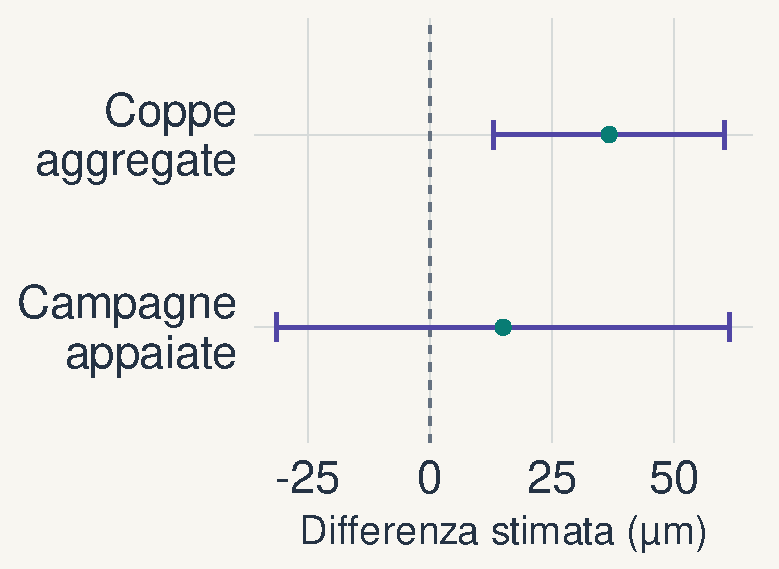
\includegraphics[width=\linewidth,height=6.15cm,keepaspectratio]{Figure/F08.pdf}\par}
\PSmall{Coppe riunite: controesempio Welch. Campagne appaiate: intervallo t sulle quattro differenze. Cambiano quantità e ipotesi.}
}};
\node[anchor=north west,inner sep=0] at([xshift=10.85cm,yshift=-2.12cm]current page.north west){\Colonna{8.16cm}{\PBody{La figura accosta il confronto sulle coppe riunite e quello sulle campagne complete, con i rispettivi intervalli classici. La differenza delle stime dipende da pesi e campagne incluse, mentre la differenza dell’incertezza riflette anche l’unità scelta e le assunzioni di indipendenza. Il risultato più netto sulle coppe non offre una ragione per preferire quella procedura. La discussione identifica prima l’oggetto della media e il disegno delle osservazioni, così da scegliere un’analisi pertinente alla domanda e dichiararne i limiti.}
}};
\end{tikzpicture}\end{frame}

\begin{frame}[plain]\hypertarget{slide17}{}
\bookmark[level=1,page=17]{Il bootstrap conserva la campagna come unità}
\begin{tikzpicture}[remember picture,overlay]
\PilotChrome{Il bootstrap conserva la campagna come unità}{INCERTEZZA CON QUATTRO UNITÀ}{17}{Il ricampionamento rende esplicita la variabilità del campione disponibile senza crearne nuove unità.}
\node[anchor=north west,inner sep=0] at([xshift=.96cm,yshift=-2.12cm]current page.north west){\Colonna{9.40cm}{{\centering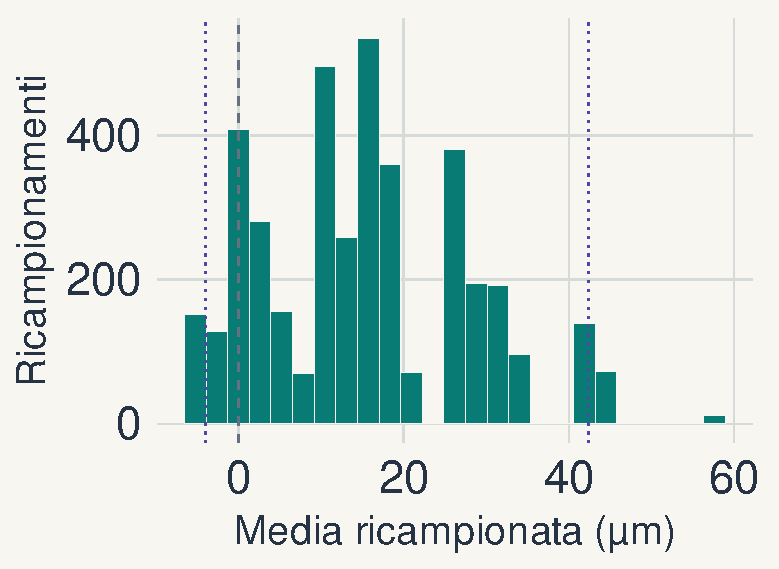
\includegraphics[width=\linewidth,height=6.15cm,keepaspectratio]{Figure/F05.pdf}\par}
\PSmall{$d_g$: differenza di campagna, in µm. 4000 estrazioni con reinserimento; viola: quantili percentili della media ricampionata.}
}};
\node[anchor=north west,inner sep=0] at([xshift=10.85cm,yshift=-2.12cm]current page.north west){\Colonna{8.16cm}{\PBody{Ogni replica estrae quattro differenze di campagna con reinserimento e ne calcola la media. I quattromila piani condivisi producono soltanto trentacinque valori distinti, perché il campione originario contiene quattro quantità e le loro combinazioni di molteplicità sono limitate. L’intervallo percentile va da circa meno 3,98 a più 42,41 micrometri. Il ricampionamento descrive la sensibilità alle campagne osservate, senza rappresentare automaticamente campagne climaticamente differenti o condizioni assenti dal sito e dal periodo considerati.}
\par\smallskip{\centering\adjustbox{max width=.98\linewidth}{$\displaystyle \bar d^*=\frac14\sum_{r=1}^{4}d_{I_r},\qquad I_r\overset{\rm iid}{\sim}\mathrm{Unif}\{1{,}2{,}3{,}4\}$}\par\smallskip}
}};
\end{tikzpicture}\end{frame}

\begin{frame}[plain]\hypertarget{slide18}{}
\bookmark[level=1,page=18]{Ribaltamento dei segni e ipotesi di simmetria}
\begin{tikzpicture}[remember picture,overlay]
\PilotChrome{Ribaltamento dei segni e ipotesi di simmetria}{INCERTEZZA CON QUATTRO UNITÀ}{18}{L’enumerazione è esatta per il riferimento scelto, la cui pertinenza al disegno osservativo deve essere motivata.}
\node[anchor=north west,inner sep=0] at([xshift=.96cm,yshift=-2.12cm]current page.north west){\Colonna{9.40cm}{{\centering\resizebox{0.90\linewidth}{!}{\begin{tikzpicture}[x=1cm,y=-.87cm,every node/.style={font=\fontsize{12.2}{15}\selectfont,text=Ink},arr/.style={-{Stealth[length=2mm]},line width=.8pt,draw=Classical}]\path[use as bounding box] (0,0) rectangle (7.45,6.2);
\draw[draw=Quantum,fill=Quantum!8,rounded corners=2pt,line width=.7pt] (0.45,0.5) rectangle (2.0,1.45);
\node[anchor=center,text=Ink,font=\fontsize{12}{15}\selectfont] at (1.225,0.975) {\texttt{----}};
\draw[draw=Classical,fill=Classical!8,rounded corners=2pt,line width=.7pt] (2.2,0.5) rectangle (3.75,1.45);
\node[anchor=center,text=Ink,font=\fontsize{12}{15}\selectfont] at (2.975,0.975) {\texttt{---+}};
\draw[draw=Quantum,fill=Quantum!8,rounded corners=2pt,line width=.7pt] (3.95,0.5) rectangle (5.5,1.45);
\node[anchor=center,text=Ink,font=\fontsize{12}{15}\selectfont] at (4.725,0.975) {\texttt{--+-}};
\draw[draw=Classical,fill=Classical!8,rounded corners=2pt,line width=.7pt] (5.7,0.5) rectangle (7.25,1.45);
\node[anchor=center,text=Ink,font=\fontsize{12}{15}\selectfont] at (6.475,0.975) {\texttt{--++}};
\draw[draw=Classical,fill=Classical!8,rounded corners=2pt,line width=.7pt] (0.45,1.8) rectangle (2.0,2.75);
\node[anchor=center,text=Ink,font=\fontsize{12}{15}\selectfont] at (1.225,2.275) {\texttt{-+--}};
\draw[draw=Quantum,fill=Quantum!8,rounded corners=2pt,line width=.7pt] (2.2,1.8) rectangle (3.75,2.75);
\node[anchor=center,text=Ink,font=\fontsize{12}{15}\selectfont] at (2.975,2.275) {\texttt{-+-+}};
\draw[draw=Classical,fill=Classical!8,rounded corners=2pt,line width=.7pt] (3.95,1.8) rectangle (5.5,2.75);
\node[anchor=center,text=Ink,font=\fontsize{12}{15}\selectfont] at (4.725,2.275) {\texttt{-++-}};
\draw[draw=Quantum,fill=Quantum!8,rounded corners=2pt,line width=.7pt] (5.7,1.8) rectangle (7.25,2.75);
\node[anchor=center,text=Ink,font=\fontsize{12}{15}\selectfont] at (6.475,2.275) {\texttt{-+++}};
\draw[draw=Quantum,fill=Quantum!8,rounded corners=2pt,line width=.7pt] (0.45,3.1) rectangle (2.0,4.05);
\node[anchor=center,text=Ink,font=\fontsize{12}{15}\selectfont] at (1.225,3.575) {\texttt{+---}};
\draw[draw=Classical,fill=Classical!8,rounded corners=2pt,line width=.7pt] (2.2,3.1) rectangle (3.75,4.05);
\node[anchor=center,text=Ink,font=\fontsize{12}{15}\selectfont] at (2.975,3.575) {\texttt{+--+}};
\draw[draw=Quantum,fill=Quantum!8,rounded corners=2pt,line width=.7pt] (3.95,3.1) rectangle (5.5,4.05);
\node[anchor=center,text=Ink,font=\fontsize{12}{15}\selectfont] at (4.725,3.575) {\texttt{+-+-}};
\draw[draw=Classical,fill=Classical!8,rounded corners=2pt,line width=.7pt] (5.7,3.1) rectangle (7.25,4.05);
\node[anchor=center,text=Ink,font=\fontsize{12}{15}\selectfont] at (6.475,3.575) {\texttt{+-++}};
\draw[draw=Classical,fill=Classical!8,rounded corners=2pt,line width=.7pt] (0.45,4.4) rectangle (2.0,5.3500000000000005);
\node[anchor=center,text=Ink,font=\fontsize{12}{15}\selectfont] at (1.225,4.875) {\texttt{++--}};
\draw[draw=Quantum,fill=Quantum!8,rounded corners=2pt,line width=.7pt] (2.2,4.4) rectangle (3.75,5.3500000000000005);
\node[anchor=center,text=Ink,font=\fontsize{12}{15}\selectfont] at (2.975,4.875) {\texttt{++-+}};
\draw[draw=Classical,fill=Classical!8,rounded corners=2pt,line width=.7pt] (3.95,4.4) rectangle (5.5,5.3500000000000005);
\node[anchor=center,text=Ink,font=\fontsize{12}{15}\selectfont] at (4.725,4.875) {\texttt{+++-}};
\draw[draw=Quantum,fill=Quantum!8,rounded corners=2pt,line width=.7pt] (5.7,4.4) rectangle (7.25,5.3500000000000005);
\node[anchor=center,text=Ink,font=\fontsize{12}{15}\selectfont] at (6.475,4.875) {\texttt{++++}};
\node[anchor=center,text=Ink,font=\fontsize{10.7}{15}\selectfont,text width=6.9cm,align=center] at (3.7,5.85) {Viola: otto esiti estremi.};

\end{tikzpicture}}\par}
\PSmall{$d_g$: differenza ottobre–marzo meno aprile–settembre nella campagna g; $s_g$: segno applicato. T(s) è la media dopo i ribaltamenti.}
}};
\node[anchor=north west,inner sep=0] at([xshift=10.85cm,yshift=-2.12cm]current page.north west){\Colonna{8.16cm}{\PBody{Un controllo ulteriore conserva le grandezze delle differenze e ne enumera i possibili segni. Con quattro differenze si ottengono sedici configurazioni, considerate equiprobabili sotto un’ipotesi di simmetria e indipendenza dei segni rispetto alla nullità dell’effetto. Nel disegno osservativo non è avvenuta una randomizzazione dei segni: l’interpretazione dipende quindi da questa ipotesi di riferimento. Otto configurazioni hanno una media in valore assoluto almeno pari a quella osservata, producendo una probabilità bilaterale di un mezzo.}
\par\smallskip{\centering\adjustbox{max width=.98\linewidth}{$\displaystyle T(s)=\frac14\sum_{g=1}^{4}s_gd_g,\qquad s_g\in\{-1,+1\}$}\par\smallskip}
}};
\end{tikzpicture}\end{frame}

\begin{frame}[plain]\hypertarget{slide19}{}
\bookmark[level=1,page=19]{La risoluzione del test dipende dal disegno}
\begin{tikzpicture}[remember picture,overlay]
\PilotChrome{La risoluzione del test dipende dal disegno}{INCERTEZZA CON QUATTRO UNITÀ}{19}{La risoluzione inferenziale deriva dal disegno e resta distinta dalla precisione aritmetica.}
\node[anchor=north west,inner sep=0] at([xshift=.96cm,yshift=-2.12cm]current page.north west){\Colonna{9.40cm}{{\centering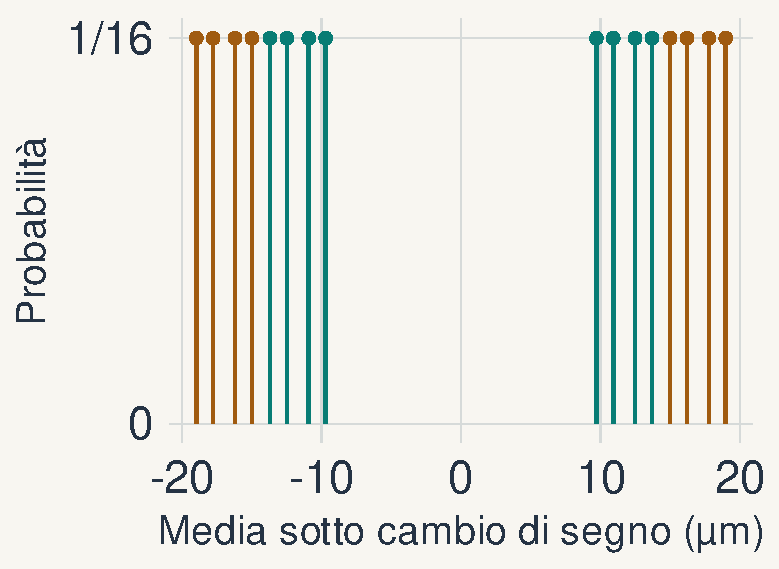
\includegraphics[width=\linewidth,height=6.15cm,keepaspectratio]{Figure/F06.pdf}\par}
\PSmall{T(s): media delle differenze con segni ribaltati; $\bar d=14,99$ µm: media osservata. Ocra: otto configurazioni almeno altrettanto estreme.}
}};
\node[anchor=north west,inner sep=0] at([xshift=10.85cm,yshift=-2.12cm]current page.north west){\Colonna{8.16cm}{\PBody{La distribuzione di riferimento contiene sedici masse di probabilità uguali a un sedicesimo. La simmetria associa a ogni configurazione quella con tutti i segni invertiti, per cui il più piccolo valore bilaterale possibile è due sedicesimi, pari a 0,125, quando le due configurazioni estreme sono uniche. Una maggiore precisione numerica del calcolo non supera questo limite, che deriva dal numero delle unità e dal riferimento utilizzato. Nel caso osservato la probabilità è 0,5, coerentemente con le otto configurazioni evidenziate.}
\par\smallskip{\centering\adjustbox{max width=.98\linewidth}{$\displaystyle p=\frac{\#\{|T(s)|\geq|\overline d|\}}{16}=\frac8{16}=0{,}5$}\par\smallskip}
}};
\end{tikzpicture}\end{frame}

\begin{frame}[plain]\hypertarget{slide20}{}
\bookmark[level=1,page=20]{Sensibilità alla singola campagna}
\begin{tikzpicture}[remember picture,overlay]
\PilotChrome{Sensibilità alla singola campagna}{INCERTEZZA CON QUATTRO UNITÀ}{20}{L’influenza di una campagna orienta il controllo del disegno e del contesto, prima di qualsiasi esclusione.}
\node[anchor=north west,inner sep=0] at([xshift=.96cm,yshift=-2.12cm]current page.north west){\Colonna{9.40cm}{{\centering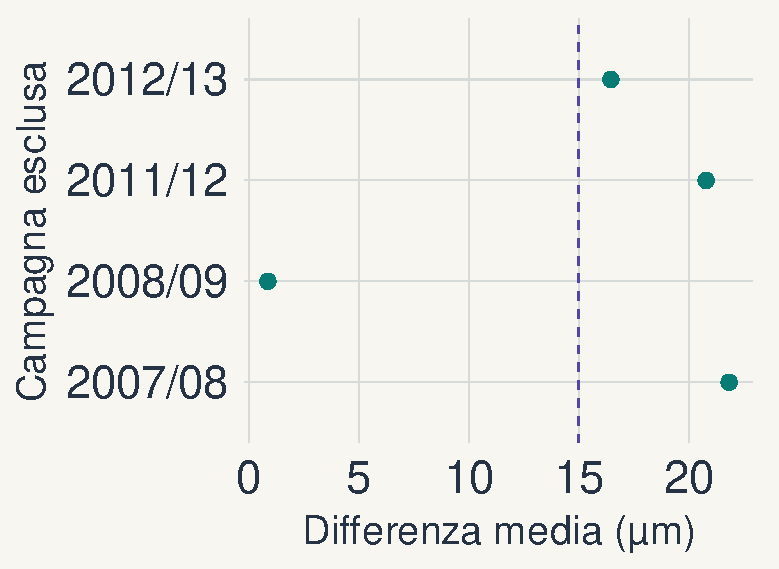
\includegraphics[width=\linewidth,height=6.15cm,keepaspectratio]{Figure/F07.pdf}\par}
\PSmall{Media delle tre differenze rimaste dopo ogni omissione. La linea viola indica la media sulle quattro campagne.}
}};
\node[anchor=north west,inner sep=0] at([xshift=10.85cm,yshift=-2.12cm]current page.north west){\Colonna{8.16cm}{\PBody{L’omissione di una campagna alla volta produce medie comprese fra circa 0,87 e 21,84 micrometri. Escludendo il 2008–2009, la differenza media si avvicina allo zero, rendendo evidente il contributo di quell’anno alla sintesi complessiva. Questa diagnosi orienta l’esame della copertura e delle condizioni ambientali, senza fornire da sola una motivazione per eliminare la campagna. La relazione deve conservare il risultato sul campione completo e discutere le alternative attraverso evidenze indipendenti dalla convenienza della conclusione.}
}};
\end{tikzpicture}\end{frame}

\begin{frame}[plain]\hypertarget{slide21}{}
\bookmark[level=0,page=21]{Interpretazione e nuova raccolta}
\bookmark[level=1,page=21]{Dal calendario alle ipotesi ambientali}
\begin{tikzpicture}[remember picture,overlay]
\PilotChrome{Dal calendario alle ipotesi ambientali}{INTERPRETAZIONE E NUOVA RACCOLTA}{21}{Il raggruppamento temporale descrive un confronto e lascia aperta l’identificazione dei meccanismi.}
\node[anchor=north west,inner sep=0] at([xshift=.96cm,yshift=-2.12cm]current page.north west){\Colonna{9.40cm}{{\centering\resizebox{0.90\linewidth}{!}{\begin{tikzpicture}[x=1cm,y=-.87cm,every node/.style={font=\fontsize{12.2}{15}\selectfont,text=Ink},arr/.style={-{Stealth[length=2mm]},line width=.8pt,draw=Classical}]\path[use as bounding box] (0,0) rectangle (7.45,6.2);
\draw[draw=Classical,fill=Classical!8,rounded corners=2pt,line width=.7pt] (0.5,0.6) rectangle (6.9,1.9);
\node[anchor=center,text=Ink,font=\fontsize{12.2}{15}\selectfont,text width=6cm,align=center] at (3.7,1.25) {Fascia calendario osservata};
\draw[arr,draw=Classical] (2,2.1)--(2,3);
\draw[arr,draw=Quantum] (5.4,2.1)--(5.4,3);
\draw[draw=Classical,fill=Classical!8,rounded corners=2pt,line width=.7pt] (0.4,3.2) rectangle (3.5,4.7);
\node[anchor=center,text=Ink,font=\fontsize{11.5}{15}\selectfont,text width=2.8cm,align=center] at (1.95,3.95) {Produzione e crescita};
\draw[draw=Quantum,fill=Quantum!8,rounded corners=2pt,line width=.7pt] (3.9,3.2) rectangle (7,4.7);
\node[anchor=center,text=Ink,font=\fontsize{11.5}{15}\selectfont,text width=2.8cm,align=center] at (5.45,3.95) {Trasporto e conservazione};
\node[anchor=center,text=Ink,font=\fontsize{11.5}{15}\selectfont,text width=6.8cm,align=center] at (3.7,5.6) {Meccanismi da distinguere con dati ulteriori};

\end{tikzpicture}}\par}
}};
\node[anchor=north west,inner sep=0] at([xshift=10.85cm,yshift=-2.12cm]current page.north west){\Colonna{8.16cm}{\PBody{Le fasce temporali possono essere associate a condizioni differenti di produzione, nutrimento, trasporto e conservazione dei gusci, ma il confronto delle medie non distingue questi meccanismi. Una sola posizione geografica e quattro campagne complete delimitano ulteriormente l’argomento. Il risultato sostiene una descrizione della differenza nelle campagne disponibili, accompagnata da un’incertezza ampia e da sensibilità fra anni. Per studiare il meccanismo servirebbero misure ambientali concomitanti e un disegno che colleghi tali variazioni alle proprietà morfometriche osservate.}
}};
\end{tikzpicture}\end{frame}

\begin{frame}[plain]\hypertarget{slide22}{}
\bookmark[level=1,page=22]{Progettare una copertura più informativa}
\begin{tikzpicture}[remember picture,overlay]
\PilotChrome{Progettare una copertura più informativa}{INTERPRETAZIONE E NUOVA RACCOLTA}{22}{La raccolta aggiuntiva va progettata rispetto alla componente di incertezza che si vuole ridurre.}
\node[anchor=north west,inner sep=0] at([xshift=.96cm,yshift=-2.12cm]current page.north west){\Colonna{9.40cm}{{\centering\resizebox{0.90\linewidth}{!}{\begin{tikzpicture}[x=1cm,y=-.87cm,every node/.style={font=\fontsize{12.2}{15}\selectfont,text=Ink},arr/.style={-{Stealth[length=2mm]},line width=.8pt,draw=Classical}]\path[use as bounding box] (0,0) rectangle (7.45,6.2);
\draw[draw=Classical,fill=Classical!8,rounded corners=2pt,line width=.7pt] (0.5,0.5) rectangle (6.9,1.8);
\node[anchor=center,text=Ink,font=\fontsize{12.2}{15}\selectfont,text width=6cm,align=center] at (3.7,1.15) {Individui: numerosità e dispersione};
\draw[draw=Quantum,fill=Quantum!8,rounded corners=2pt,line width=.7pt] (0.5,2.5) rectangle (6.9,3.8);
\node[anchor=center,text=Ink,font=\fontsize{12.2}{15}\selectfont,text width=6cm,align=center] at (3.7,3.15) {Coppe: durata, copertura e flusso};
\draw[draw=Measure,fill=Measure!8,rounded corners=2pt,line width=.7pt] (0.5,4.5) rectangle (6.9,5.8);
\node[anchor=center,text=Ink,font=\fontsize{11.5}{15}\selectfont,text width=6cm,align=center] at (3.7,5.15) {Campagne e siti: nuove unità di confronto};

\end{tikzpicture}}\par}
}};
\node[anchor=north west,inner sep=0] at([xshift=10.85cm,yshift=-2.12cm]current page.north west){\Colonna{8.16cm}{\PBody{Una raccolta successiva dovrebbe migliorare la copertura delle due fasce in più campagne, documentando intervalli di apertura delle coppe, numero di individui, dispersione delle misure e flusso sedimentario. Queste informazioni permetterebbero di definire ponderazioni coerenti con la quantità scientifica di interesse e di separare l’incertezza interna alle coppe dalla variabilità fra campagne. Ulteriori siti amplierebbero il dominio geografico, purché la loro selezione e i protocolli fossero comparabili. Il miglioramento del disegno riguarda pertanto livelli diversi della gerarchia osservativa.}
}};
\end{tikzpicture}\end{frame}

\begin{frame}[plain]\hypertarget{slide23}{}
\bookmark[level=1,page=23]{Relazione e discussione del confronto}
\begin{tikzpicture}[remember picture,overlay]
\PilotChrome{Relazione e discussione del confronto}{INTERPRETAZIONE E NUOVA RACCOLTA}{23}{La relazione sostiene la conclusione attraverso il disegno osservativo, oltre che attraverso i risultati numerici.}
\node[anchor=north west,inner sep=0] at([xshift=.96cm,yshift=-2.12cm]current page.north west){\Colonna{9.40cm}{\PBody{La consegna include matrice della copertura, grafico delle coppie, definizione della differenza, intervallo t, bootstrap, controllo dei segni e sensibilità alle campagne. L’esercizio confronta il risultato sulle coppe riunite con quello appaiato, spiegando come cambino pesi, campione e assunzioni. Una risposta adeguata mantiene distinti assenza di evidenza netta, equivalenza fra fasce e identificazione di un meccanismo. Codice, dati e attribuzioni consentono di ricostruire il procedimento e di proporre una nuova raccolta coerente con i limiti emersi.}
}};
\node[anchor=north west,inner sep=0] at([xshift=10.85cm,yshift=-2.12cm]current page.north west){\Colonna{8.16cm}{\PInfo{R/P02\_figure.R produce le figure e le tabelle a partire dall’estratto conservato in dati/progetti. La fonte è Mikis et al. (2019), PANGAEA.902776, distribuita con licenza CC BY 4.0. Il progetto raccorda campionamento gerarchico, inferenza sulla media e test appaiati dei moduli M01, M05 e M06.}
}};
\end{tikzpicture}\end{frame}

\begin{frame}[plain]\hypertarget{slide24}{}
\bookmark[level=0,page=24]{Laboratori della spedizione}
\bookmark[level=1,page=24]{Tre fasi della spedizione nel laboratorio}
\begin{tikzpicture}[remember picture,overlay]
\PilotChrome{Tre fasi della spedizione nel laboratorio}{LABORATORI DELLA SPEDIZIONE}{24}{Gli esperimenti usano dati sintetici; la conclusione sul caso resta quella ottenuta dalle quattro campagne.}
\node[anchor=north west,inner sep=0] at([xshift=.96cm,yshift=-2.12cm]current page.north west){\Colonna{9.40cm}{{\centering\resizebox{0.97\linewidth}{!}{\begin{tikzpicture}[x=1cm,y=1cm,every node/.style={font=\sffamily\fontsize{9.2}{11}\selectfont,text=Ink}]
\node[draw=Classical,fill=Classical,rounded corners=2mm,text=white,text width=2.45cm,align=flush center,minimum height=1.55cm,anchor=west,font=\sffamily\bfseries\fontsize{9.2}{11}\selectfont] (f0) at (0,0.00) {1. Delimitare il confronto};
\node[draw=Classical!60,fill=Classical!6,rounded corners=1.5mm,line width=.6pt,text width=2.8cm,align=flush center,minimum height=1.55cm,anchor=west] (e00) at (2.95,0.00) {Definire la quantità di interesse\\[1pt]{\fontsize{7.6}{9}\selectfont\color{Muted}m01-estimando}};
\node[draw=Rule,fill=white,rounded corners=1.5mm,line width=.6pt,text width=2.8cm,align=flush center,minimum height=1.55cm,anchor=west] (e01) at (6.10,0.00) {Aggregazione e pesi delle osservazioni\\[1pt]{\fontsize{7.6}{9}\selectfont\color{Muted}m02-aggregazioni}};
\draw[pEdge] (f0.east)--(e00.west);
\node[draw=Classical,fill=Classical,rounded corners=2mm,text=white,text width=2.45cm,align=flush center,minimum height=1.55cm,anchor=west,font=\sffamily\bfseries\fontsize{9.2}{11}\selectfont] (f1) at (0,-1.95) {2. Valutare l’incertezza};
\draw[pEdge] (f0.south)--(f1.north);
\node[draw=Classical!60,fill=Classical!6,rounded corners=1.5mm,line width=.6pt,text width=2.8cm,align=flush center,minimum height=1.55cm,anchor=west] (e10) at (2.95,-1.95) {Definire un contrasto fra gruppi\\[1pt]{\fontsize{7.6}{9}\selectfont\color{Muted}m06-contrasto}};
\node[draw=Rule,fill=white,rounded corners=1.5mm,line width=.6pt,text width=2.8cm,align=flush center,minimum height=1.55cm,anchor=west] (e11) at (6.10,-1.95) {Ricampionamento per stazioni\\[1pt]{\fontsize{7.6}{9}\selectfont\color{Muted}m05-ricampionamento}};
\draw[pEdge] (f1.east)--(e10.west);
\node[draw=Classical,fill=Classical,rounded corners=2mm,text=white,text width=2.45cm,align=flush center,minimum height=1.55cm,anchor=west,font=\sffamily\bfseries\fontsize{9.2}{11}\selectfont] (f2) at (0,-3.90) {3. Preparare una nuova raccolta};
\draw[pEdge] (f1.south)--(f2.north);
\node[draw=Classical!60,fill=Classical!6,rounded corners=1.5mm,line width=.6pt,text width=2.8cm,align=flush center,minimum height=1.55cm,anchor=west] (e20) at (2.95,-3.90) {Disegnare una campagna di misura\\[1pt]{\fontsize{7.6}{9}\selectfont\color{Muted}m01-disegno}};
\node[draw=Rule,fill=white,rounded corners=1.5mm,line width=.6pt,text width=2.8cm,align=flush center,minimum height=1.55cm,anchor=west] (e21) at (6.10,-3.90) {Confrontare campagne ripetute\\[1pt]{\fontsize{7.6}{9}\selectfont\color{Muted}m01-confronto-disegni}};
\draw[pEdge] (f2.east)--(e20.west);
\end{tikzpicture}
}\par}
\PSmall{Fasi della spedizione. Il primo esperimento di ogni fase ha le pagine Scenario A e Confronto.}
}};
\node[anchor=north west,inner sep=0] at([xshift=10.85cm,yshift=-2.12cm]current page.north west){\Colonna{8.16cm}{\PBody{Gli esperimenti ripetono su dati sintetici tre scelte della spedizione: quale quantità sintetizzare, come costruire un contrasto fra gruppi, quale disegno dare a una nuova campagna. Ogni fase ha uno scenario di partenza e un confronto con un solo parametro modificato.}
\vspace{.2cm}\PLabel{Altri esperimenti delle fasi}
\PLab{https://marzione00.github.io/Lab_Geo/\#laboratorio/m02-aggregazioni}{Aggregazione e pesi delle osservazioni · m02-aggregazioni}
\PLab{https://marzione00.github.io/Lab_Geo/\#laboratorio/m05-ricampionamento}{Ricampionamento per stazioni · m05-ricampionamento}
\PLab{https://marzione00.github.io/Lab_Geo/\#laboratorio/m01-confronto-disegni}{Confrontare campagne ripetute · m01-confronto-disegni}
}};
\end{tikzpicture}\end{frame}

\begin{frame}[plain]\hypertarget{slide25}{}
\bookmark[level=1,page=25]{Definire la quantità di interesse}
\begin{tikzpicture}[remember picture,overlay]
\PilotChrome{Definire la quantità di interesse}{LABORATORI DELLA SPEDIZIONE}{25}{Distinguere media delle misure e media delle unità geologiche.}
\node[anchor=north west,inner sep=0] at([xshift=.96cm,yshift=-2.12cm]current page.north west){\Colonna{9.40cm}{{\centering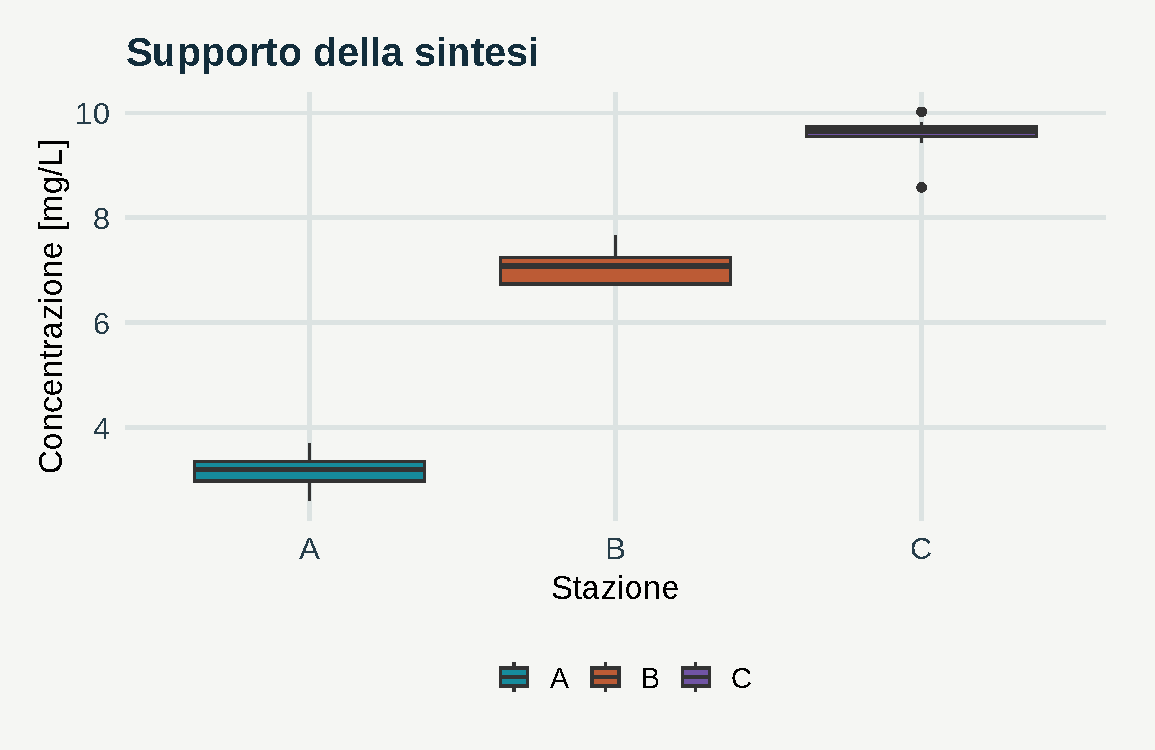
\includegraphics[width=\linewidth,height=6.0cm,keepaspectratio]{Esperimenti/m01-estimando-A.pdf}\par}
\PSmall{Misure nella stazione A: 20. Seme: 17.}
}};
\node[anchor=north west,inner sep=0] at([xshift=10.85cm,yshift=-2.12cm]current page.north west){\Colonna{8.16cm}{\PLabel{Scenario A · simulazione}
\PBody{Le stazioni rappresentano unità geologiche con concentrazioni medie differenti. Aumentando il numero di misure nella prima stazione, cresce il suo peso nella media complessiva delle osservazioni, mentre la media delle medie assegna lo stesso peso a ciascuna stazione, indipendentemente dall’intensità della raccolta.}
\par\smallskip{\centering\adjustbox{max width=.98\linewidth}{$\displaystyle \bar x_{\rm misure}=\frac{\sum_g n_g\bar x_g}{\sum_g n_g},\quad \bar x_{\rm stazioni}=G^{-1}\sum_g\bar x_g$}\par\smallskip}
\PSmall{$g$ identifica la stazione; $n_g$ ne indica la numerosità; $\bar x_g$ è la sua media campionaria; $G$ è il numero delle stazioni.}
}};
\node[anchor=north east,inner sep=0] at([xshift=17.1cm,yshift=-12.04cm]current page.north west){\fontsize{7.7}{9}\selectfont \href{https://marzione00.github.io/Lab_Geo/\#laboratorio/m01-estimando}{\color{Classical}\bfseries Apri il laboratorio · m01-estimando}};
\end{tikzpicture}\end{frame}

\begin{frame}[plain]\hypertarget{slide26}{}
\bookmark[level=1,page=26]{Confronto | Definire la quantità di interesse}
\begin{tikzpicture}[remember picture,overlay]
\PilotChrome{Confronto | Definire la quantità di interesse}{LABORATORI DELLA SPEDIZIONE}{26}{Il peso attribuito a ogni unità determina la quantità sintetizzata.}
\node[anchor=north west,inner sep=0] at([xshift=.96cm,yshift=-2.12cm]current page.north west){\Colonna{9.40cm}{{\centering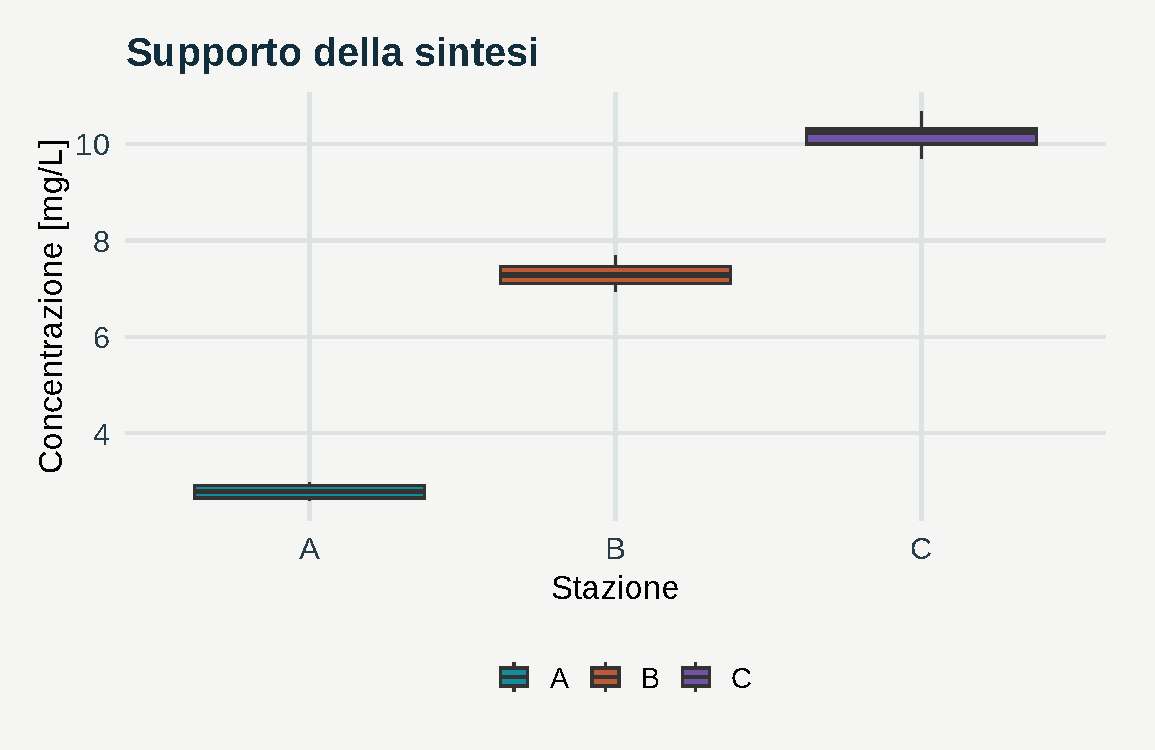
\includegraphics[width=\linewidth,height=5.6cm,keepaspectratio]{Esperimenti/m01-estimando-B.pdf}\par}
\PSmall{Misure nella stazione A: 20 $\to$ 4. Tutti gli altri parametri e il seme sono fissi.}
}};
\node[anchor=north west,inner sep=0] at([xshift=10.85cm,yshift=-2.12cm]current page.north west){\Colonna{8.16cm}{\PLabel{Confronto fra gli scenari}
{\fontsize{10.2}{12.8}\selectfont\begin{tabular}{@{}>{\raggedright\arraybackslash}p{0.48\linewidth}@{\hspace{.13cm}}>{\raggedright\arraybackslash}p{0.224\linewidth}@{\hspace{.13cm}}>{\raggedright\arraybackslash}p{0.224\linewidth}@{}}\toprule Grandezza & A & B\\[2.3pt]
\midrule 
Media delle misure & 5,75 & 7,75\\[2.3pt]
Media delle stazioni & 6,61 & 6,75\\[2.3pt]
\bottomrule\end{tabular}\par}
\vspace{.25cm}\PBody{Con quattro sole misure nella stazione A la media delle misure sale da 5,75 a 7,75, perché la stazione con valori bassi pesa meno; la media delle stazioni passa da 6,61 a 6,75. Nella spedizione lo stesso meccanismo assegna più peso alle campagne con più coppe.}
}};
\node[anchor=north east,inner sep=0] at([xshift=17.1cm,yshift=-12.04cm]current page.north west){\fontsize{7.7}{9}\selectfont \href{https://marzione00.github.io/Lab_Geo/\#laboratorio/m01-estimando}{\color{Classical}\bfseries Apri il laboratorio · m01-estimando}};
\end{tikzpicture}\end{frame}

\begin{frame}[plain]\hypertarget{slide27}{}
\bookmark[level=1,page=27]{Definire un contrasto fra gruppi}
\begin{tikzpicture}[remember picture,overlay]
\PilotChrome{Definire un contrasto fra gruppi}{LABORATORI DELLA SPEDIZIONE}{27}{Collegare disegno e differenza di interesse.}
\node[anchor=north west,inner sep=0] at([xshift=.96cm,yshift=-2.12cm]current page.north west){\Colonna{9.40cm}{{\centering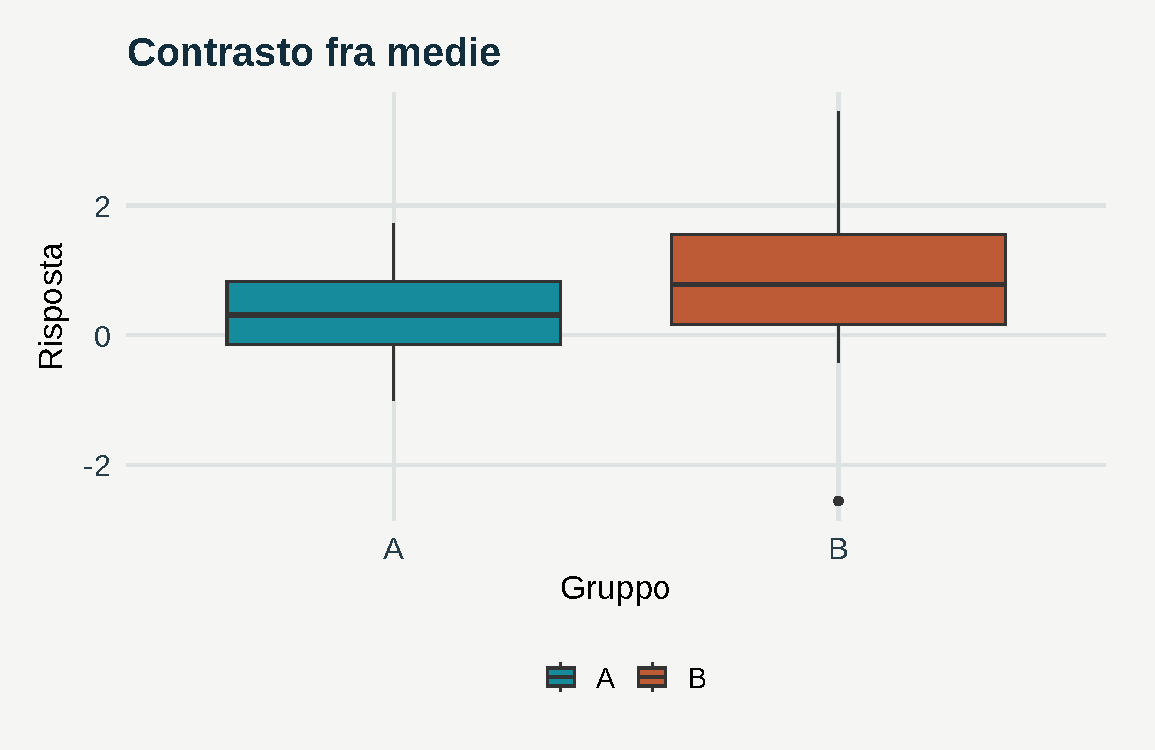
\includegraphics[width=\linewidth,height=5.0cm,keepaspectratio]{Esperimenti/m06-contrasto-A.pdf}\par}
\PSmall{Numero di osservazioni: 30. Seme: 17.}
\PSmall{$\mu_A$ e $\mu_B$ sono le medie delle popolazioni; $\Delta$ è la loro differenza. $\bar y_A$ e $\bar y_B$ sono le medie campionarie, dalle quali si ottiene la stima $\widehat\Delta$.}
}};
\node[anchor=north west,inner sep=0] at([xshift=10.85cm,yshift=-2.12cm]current page.north west){\Colonna{8.16cm}{\PLabel{Scenario A · simulazione}
\PBody{Il confronto riguarda due popolazioni normali dalle quali vengono estratti campioni indipendenti di uguale numerosità. La differenza impostata nel pannello sposta la media della popolazione B, mentre la dispersione delle due popolazioni rimane unitaria. Poiché le medie campionarie risentono del caso, il contrasto osservato può discostarsi dalla differenza utilizzata per generare i dati.}
\par\smallskip{\centering\adjustbox{max width=.98\linewidth}{$\displaystyle \Delta=\mu_B-\mu_A,\quad\widehat\Delta=\bar y_B-\bar y_A$}\par\smallskip}
}};
\node[anchor=north east,inner sep=0] at([xshift=17.1cm,yshift=-12.04cm]current page.north west){\fontsize{7.7}{9}\selectfont \href{https://marzione00.github.io/Lab_Geo/\#laboratorio/m06-contrasto}{\color{Classical}\bfseries Apri il laboratorio · m06-contrasto}};
\end{tikzpicture}\end{frame}

\begin{frame}[plain]\hypertarget{slide28}{}
\bookmark[level=1,page=28]{Confronto | Definire un contrasto fra gruppi}
\begin{tikzpicture}[remember picture,overlay]
\PilotChrome{Confronto | Definire un contrasto fra gruppi}{LABORATORI DELLA SPEDIZIONE}{28}{Il contrasto e le unità indipendenti precedono la scelta del test.}
\node[anchor=north west,inner sep=0] at([xshift=.96cm,yshift=-2.12cm]current page.north west){\Colonna{9.40cm}{{\centering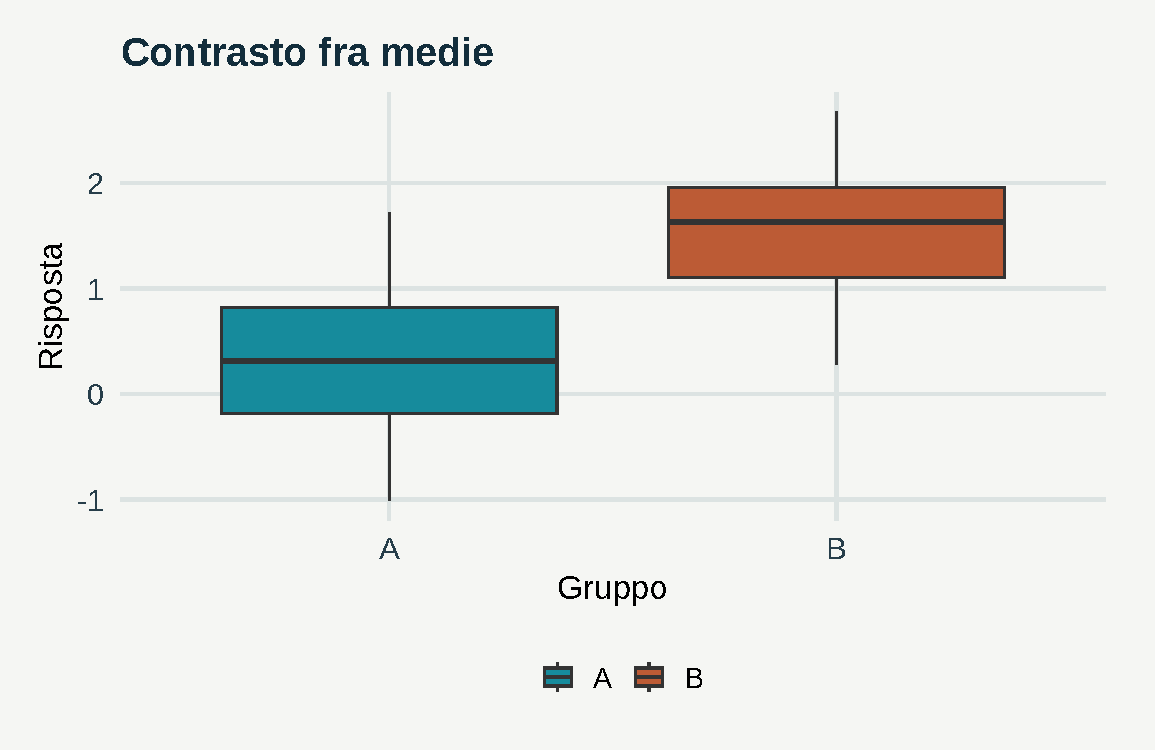
\includegraphics[width=\linewidth,height=5.6cm,keepaspectratio]{Esperimenti/m06-contrasto-B.pdf}\par}
\PSmall{Numero di osservazioni: 30 $\to$ 12. Tutti gli altri parametri e il seme sono fissi.}
}};
\node[anchor=north west,inner sep=0] at([xshift=10.85cm,yshift=-2.12cm]current page.north west){\Colonna{8.16cm}{\PLabel{Confronto fra gli scenari}
{\fontsize{10.2}{12.8}\selectfont\begin{tabular}{@{}>{\raggedright\arraybackslash}p{0.48\linewidth}@{\hspace{.13cm}}>{\raggedright\arraybackslash}p{0.224\linewidth}@{\hspace{.13cm}}>{\raggedright\arraybackslash}p{0.224\linewidth}@{}}\toprule Grandezza & A & B\\[2.3pt]
\midrule 
Differenza stimata & 0,603 & 1,22\\[2.3pt]
Limite inferiore & 0,0631 & 0,544\\[2.3pt]
Limite superiore & 1,14 & 1,89\\[2.3pt]
\bottomrule\end{tabular}\par}
\vspace{.25cm}\PBody{Con dodici osservazioni l’intervallo si allarga da 1,08 a 1,35 unità e la differenza stimata passa da 0,603 a 1,22: con poche unità anche la stima puntuale oscilla di più attorno alla differenza vera, pari a 1.}
}};
\node[anchor=north east,inner sep=0] at([xshift=17.1cm,yshift=-12.04cm]current page.north west){\fontsize{7.7}{9}\selectfont \href{https://marzione00.github.io/Lab_Geo/\#laboratorio/m06-contrasto}{\color{Classical}\bfseries Apri il laboratorio · m06-contrasto}};
\end{tikzpicture}\end{frame}

\begin{frame}[plain]\hypertarget{slide29}{}
\bookmark[level=1,page=29]{Disegnare una campagna di misura}
\begin{tikzpicture}[remember picture,overlay]
\PilotChrome{Disegnare una campagna di misura}{LABORATORI DELLA SPEDIZIONE}{29}{Valutare la copertura di una raccolta su un territorio sintetico.}
\node[anchor=north west,inner sep=0] at([xshift=.96cm,yshift=-2.12cm]current page.north west){\Colonna{9.40cm}{{\centering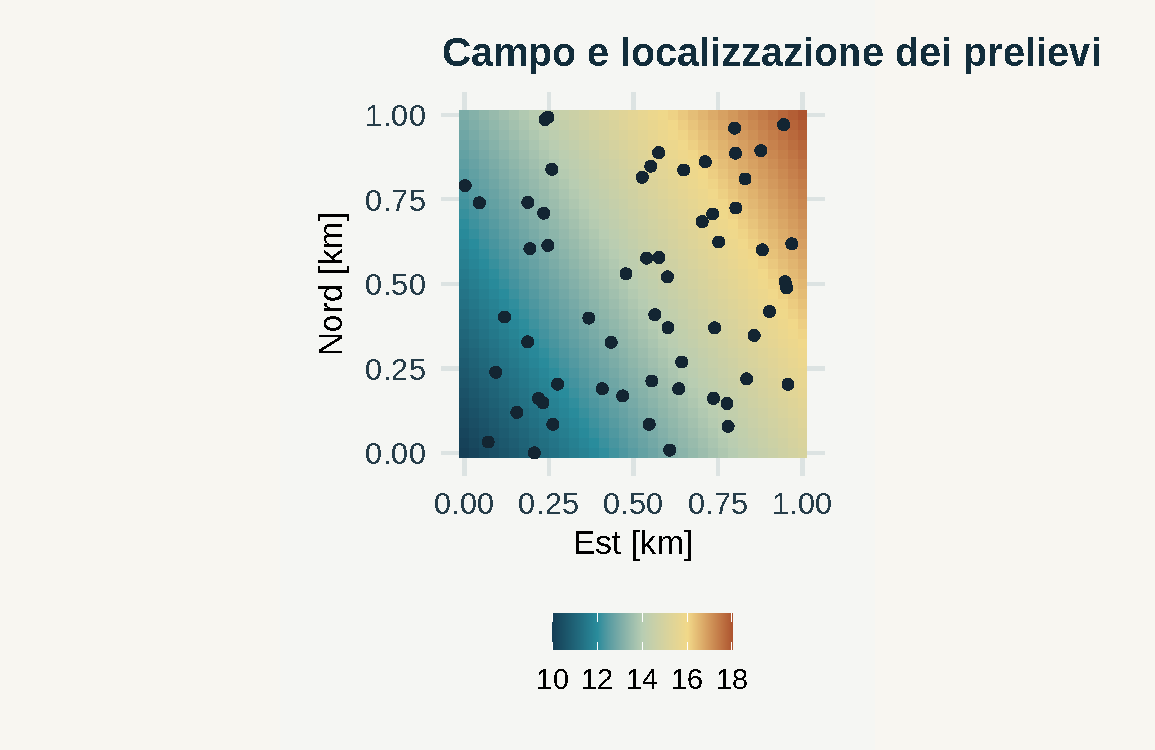
\includegraphics[width=\linewidth,height=5.0cm,keepaspectratio]{Esperimenti/m01-disegno-A.pdf}\par}
\PSmall{Disegno: Casuale. Seme: 17.}
\PSmall{$s_i$ è la posizione del prelievo; $z(s_i)$ è il valore del campo in quel punto; $n$ è il numero effettivo dei prelievi; $\widehat\mu$ è la loro media.}
}};
\node[anchor=north west,inner sep=0] at([xshift=10.85cm,yshift=-2.12cm]current page.north west){\Colonna{8.16cm}{\PLabel{Scenario A · simulazione}
\PBody{Il territorio sintetico contiene un campo che varia progressivamente lungo entrambe le coordinate. La raccolta casuale distribuisce i punti nel dominio, mentre la raccolta lungo una strada li concentra in una fascia limitata. La griglia propone una disposizione regolare, la cui copertura deve essere valutata osservando le posizioni effettive.}
\par\smallskip{\centering\adjustbox{max width=.98\linewidth}{$\displaystyle \widehat\mu=n^{-1}\sum_i z(s_i)$}\par\smallskip}
}};
\node[anchor=north east,inner sep=0] at([xshift=17.1cm,yshift=-12.04cm]current page.north west){\fontsize{7.7}{9}\selectfont \href{https://marzione00.github.io/Lab_Geo/\#laboratorio/m01-disegno}{\color{Classical}\bfseries Apri il laboratorio · m01-disegno}};
\end{tikzpicture}\end{frame}

\begin{frame}[plain]\hypertarget{slide30}{}
\bookmark[level=1,page=30]{Confronto | Disegnare una campagna di misura}
\begin{tikzpicture}[remember picture,overlay]
\PilotChrome{Confronto | Disegnare una campagna di misura}{LABORATORI DELLA SPEDIZIONE}{30}{La distribuzione geografica del campione determina quali porzioni del territorio sono osservate.}
\node[anchor=north west,inner sep=0] at([xshift=.96cm,yshift=-2.12cm]current page.north west){\Colonna{9.40cm}{{\centering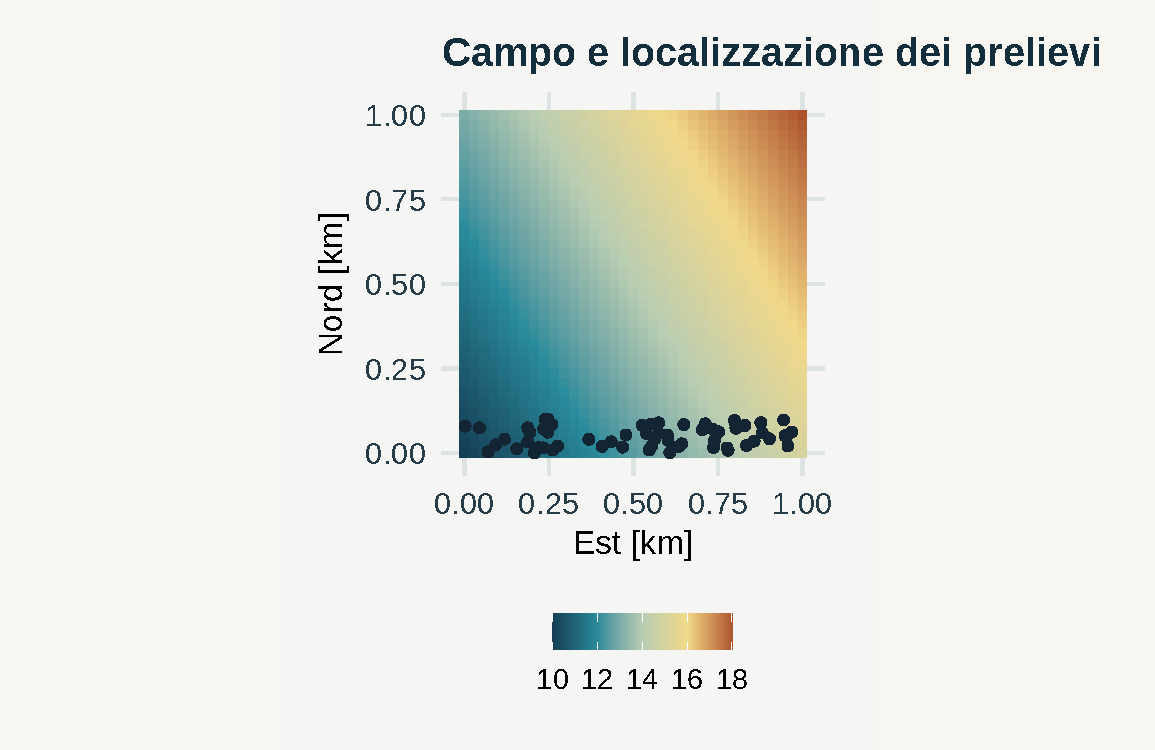
\includegraphics[width=\linewidth,height=5.6cm,keepaspectratio]{Esperimenti/m01-disegno-B.pdf}\par}
\PSmall{Disegno: Casuale $\to$ Lungo la strada. Tutti gli altri parametri e il seme sono fissi.}
}};
\node[anchor=north west,inner sep=0] at([xshift=10.85cm,yshift=-2.12cm]current page.north west){\Colonna{8.16cm}{\PLabel{Confronto fra gli scenari}
{\fontsize{10.2}{12.8}\selectfont\begin{tabular}{@{}>{\raggedright\arraybackslash}p{0.48\linewidth}@{\hspace{.13cm}}>{\raggedright\arraybackslash}p{0.224\linewidth}@{\hspace{.13cm}}>{\raggedright\arraybackslash}p{0.224\linewidth}@{}}\toprule Grandezza & A & B\\[2.3pt]
\midrule 
Media del campo & 14 & 14\\[2.3pt]
Media campionaria & 14,1 & 12,8\\[2.3pt]
Scarto & 0,136 & -1,18\\[2.3pt]
\bottomrule\end{tabular}\par}
\vspace{.25cm}\PBody{Con il campionamento lungo la strada la media campionaria scende a 12,8 contro una media del campo di 14, con uno scarto di −1,18 al posto di 0,136. Un disegno di comodo copre una parte del territorio, e il numero di osservazioni non corregge la distorsione.}
}};
\node[anchor=north east,inner sep=0] at([xshift=17.1cm,yshift=-12.04cm]current page.north west){\fontsize{7.7}{9}\selectfont \href{https://marzione00.github.io/Lab_Geo/\#laboratorio/m01-disegno}{\color{Classical}\bfseries Apri il laboratorio · m01-disegno}};
\end{tikzpicture}\end{frame}

\begin{frame}[plain]\hypertarget{slide31}{}
\bookmark[level=1,page=31]{Dal risultato alla relazione}
\begin{tikzpicture}[remember picture,overlay]
\PilotChrome{Dal risultato alla relazione}{SINTESI}{31}{Riporta differenza, unità, numero di campagne e intervallo, distinguendo assenza di evidenza netta ed equivalenza fra le fasce.}
\node[anchor=north west,inner sep=0] at([xshift=.96cm,yshift=-2.12cm]current page.north west){\Colonna{9.40cm}{\PLabel{Domanda di partenza}
\PBody{La taglia di Neogloboquadrina pachyderma cambia fra le fasce ottobre–marzo e aprile–settembre?}
\PLabel{Risultato da discutere}
\PBody{Sulle quattro campagne appaiate la differenza media fra ottobre–marzo e aprile–settembre è circa 15,0 µm, con intervallo t da −31,3 a 61,3 µm su tre gradi di libertà. Le coppe riunite darebbero 36,7 µm con p circa 0,004, perché trattano ogni coppa come unità indipendente.}
}};
\node[anchor=north west,inner sep=0] at([xshift=10.85cm,yshift=-2.12cm]current page.north west){\Colonna{8.16cm}{\PLabel{Limiti della conclusione}
\PBody{Quattro campagne, una sola trappola a 170 metri e fasce calendario definite a priori delimitano la conclusione. Escludendo la campagna 2008-2009 la stima scende a 0,87 µm, per cui la grandezza della differenza dipende soprattutto da una sola unità.}
\vspace{.4cm}\href{https://marzione00.github.io/Lab_Geo/\#modulo-P03}{\color{Classical}\bfseries Prosegui · P03 · Il Nilo: livelli e dipendenza temporale}
}};
\end{tikzpicture}\end{frame}

\begin{frame}[plain]\hypertarget{slide32}{}
\bookmark[level=1,page=32]{Fonti, dati e codice per riprodurre le figure}
\begin{tikzpicture}[remember picture,overlay]
\PilotChrome{Fonti, dati e codice per riprodurre le figure}{RIFERIMENTI}{32}{I risultati numerici si riferiscono ai dati e alle ipotesi dichiarate nel caso.}
\node[anchor=north west,inner sep=0] at([xshift=.96cm,yshift=-2.12cm]current page.north west){\Colonna{9.40cm}{\PLabel{Dati e attribuzioni}
\PBody{Estratto PANGAEA.902776, con licenza CC BY 4.0, del supplemento di Mikis e collaboratori (2019): diametri di Neogloboquadrina pachyderma in coppe di una trappola sedimentaria della Penisola Antartica occidentale.}
}};
\node[anchor=north west,inner sep=0] at([xshift=10.85cm,yshift=-2.12cm]current page.north west){\Colonna{8.16cm}{\PLabel{Nell’archivio dei sorgenti}
\PBody{Codice contiene i frammenti delle pagine; R contiene lo script P02\_figure.R, che ricostruisce figure e valori dai dati. Esperimenti comprende i programmi dei due scenari, Diagrammi i disegni TikZ modificabili, Scena il modello Blender della copertina.}
\vspace{.4cm}\href{https://marzione00.github.io/Lab_Geo/\#modulo-P02}{\color{Classical}\bfseries Apri la spedizione P02 su GeoStat Lab}
}};
\end{tikzpicture}\end{frame}
\end{document}
